\documentclass[11pt,a4paper]{article}
\usepackage[margin=1in]{geometry}
\usepackage{graphicx}
\usepackage{booktabs}
\usepackage{amsmath}
\usepackage{hyperref}
\usepackage{xcolor}
\usepackage{caption}
\usepackage{subcaption}
\usepackage{float}

\newcommand{\se}[1]{{\,\scriptstyle\pm#1}}

\title{RankAlign Training Dynamics Analysis\\
\large When Does RankAlign / TC Improve? --- \textbf{Per-Problem Fix}}
\author{Automated Analysis Report}
\date{June 21, 2026}

\begin{document}
\maketitle

\begin{abstract}
This report analyzes training dynamics for RankAlign models across four model/task combinations (gemma-2-9b-it and Qwen3.5-9B on membership and IFEval tasks). We characterize \textbf{(a)} when RankAlign improves correlation over the base model, \textbf{(b)} when the full method improves over basic RankAlign, and \textbf{(c)} when typicality correction (TC) specifically improves over non-TC training. We also report training diagnostics from WandB logs and additional statistics (concordance, score delta distributions).

\medskip
\noindent\textbf{This is the per-problem fix of the original report.} The original computed each
headline metric (gen ROC AUC, concordance, Spearman, Pearson) by pooling \emph{all} candidates for
a (model, task, setting, epoch) into one set and taking a single statistic, which conflates
problems of differing difficulty and typicality baseline. Here every headline metric is computed
\textbf{per problem, then averaged across problems, with a standard error}
($\textrm{SE}=\textrm{std}_{\textrm{ddof=1}}/\sqrt{n_{\textrm{problems}}}$). The problem unit is the
IFEval \emph{prompt} (79 train prompts, 40 candidates each) and the membership \emph{category} (68
categories, 18--96 candidates each). Loss-based sections (WandB curves, loss-component breakdown,
held-out validation loss) are unchanged --- they were never pooled-ROC metrics.
\end{abstract}

\section{Methodology: Per-Problem Aggregation}
\label{sec:perproblem-method}

For each problem $p$ (an IFEval prompt or a membership category) we take that problem's own
candidate completions and compute the metric over them: gen ROC AUC ranks the problem's correct
vs.\ incorrect candidates by the typicality-corrected generator score; concordance is the fraction
of candidate pairs whose generator and validator score differences share sign; Spearman/Pearson
correlate generator and validator scores across the problem's candidates. We then report the mean
over problems with $\textrm{SE}=\textrm{std}_{\textrm{ddof=1}}/\sqrt{n_{\textrm{problems}}}$. This
controls for the fact that different prompts/categories sit at different absolute score levels;
pooling them yields a single global AUC that does not reflect within-problem ranking quality. The
recomputation reuses the existing per-cell score files (which already carry the grouping column);
no re-evaluation was needed. Pipeline: \texttt{analysis/scripts/build\_report\_fix\_metrics.py}
(tables) and \texttt{build\_report\_fix\_figures.py} (figures), both reusing the file/setting
matching from \texttt{analyze\_all\_combos.py} and reading
\texttt{/datastor2/jdr/rankalign/outputs-trainset-dynamics/}. The figures use the \emph{same}
per-problem procedure as the HumanEval report (\texttt{build\_he\_report\_figures.py}): the
unified gen-ROC and concordance bars, the TC comparison, the per-epoch dynamics, and the
score-delta histograms are all per-problem (the generator--validator scatter pools raw candidate
points in both reports). Only the WandB loss curves and the held-out validation-loss section are
unchanged.

\paragraph{Effect of the fix.} The membership numbers barely move (categories are already
homogeneous), but the IFEval numbers rise substantially once prompts are no longer pooled (e.g.\
Gemma/IFEval base $0.670\!\to\!0.792$; Qwen/IFEval s4 $0.743\!\to\!0.858$): controlling for the
per-prompt score baseline reveals stronger within-prompt ranking than the pooled AUC suggested. One
ordering changes --- on Gemma/IFEval, s3 and s4 are now statistically tied (Section~\ref{sec:q1}).

\tableofcontents
\newpage

%% ============================================================
\section{Q1: When Does Each Component Help?}
\label{sec:q1}
%% ============================================================

\subsection{Main Comparison: Gen ROC AUC (TC, Self-Scoring)}

Table~\ref{tab:main_comparison} shows the generator ROC AUC (typicality-corrected) for the final
model (epoch 2) evaluated on the training set with self-TC scoring, computed \textbf{per problem
then averaged} (mean$\pm$SE over problems; columns: base, s1 SFT, s2 RA-basic, s3 RA-full, s4
TC-self). Bold = best per row.

\begin{table}[H]
\centering
\caption{Generator ROC AUC (TC, self-scoring) at epoch 2, per-problem mean$\pm$SE. Bold = best per
row. (Original pooled values: Gemma/Mem 0.851/0.941/0.948/0.976; Gemma/IFEval
0.670/0.586/0.482/0.753/0.801; Qwen/Mem 0.799/0.902/0.880/0.899/0.969; Qwen/IFEval
0.606/0.599/0.558/0.711/0.743.)}
\label{tab:main_comparison}
% Auto-generated by build_report_fix_metrics.py. metric=gen_roc
\begin{tabular}{lccccc}
\toprule
\textbf{Model / Task} & \textbf{Base} & \textbf{s1} & \textbf{s2} & \textbf{s3} & \textbf{s4} \\
\midrule
Gemma / Membership & $0.860\se{0.014}$ & --- & $0.945\se{0.007}$ & $0.947\se{0.011}$ & $\mathbf{0.974}\se{0.009}$ \\
Gemma / IFEval & $0.792\se{0.018}$ & $0.646\se{0.025}$ & $0.491\se{0.022}$ & $\mathbf{0.841}\se{0.016}$ & $0.837\se{0.016}$ \\
Qwen / Membership & $0.806\se{0.016}$ & $0.908\se{0.011}$ & $0.880\se{0.011}$ & $0.896\se{0.008}$ & $\mathbf{0.975}\se{0.004}$ \\
Qwen / IFEval & $0.705\se{0.019}$ & $0.685\se{0.023}$ & $0.725\se{0.019}$ & $0.843\se{0.016}$ & $\mathbf{0.858}\se{0.015}$ \\
\bottomrule
\end{tabular}

\end{table}

\subsection{Key Findings}

\begin{enumerate}
\item \textbf{s4 (TC-self) is the best, or statistically tied for best, in every combination.}
Under per-problem averaging it is strictly best in 3 of 4 cells; on Gemma/IFEval s3 ($0.841\se{0.016}$) and s4 ($0.837\se{0.016}$) are tied within one SE. (The original pooled numbers showed s4 strictly ahead everywhere; per problem the IFEval s3/s4 gap closes.)
\item \textbf{Basic RankAlign (s2) hurts on IFEval} --- Gemma/IFEval drops from $0.792$ (base) to $0.491$ (s2, $\approx$chance). Without NLL constraints, generator scores explode.
\item \textbf{The full method (s3) consistently helps}, adding large gains over base on every combo (e.g.\ Gemma/IFEval $0.792\!\to\!0.841$, Qwen/IFEval $0.705\!\to\!0.843$).
\item \textbf{TC-self (s4) adds a further gain over s3 on 3 of 4 cells} (membership and Qwen/IFEval); on Gemma/IFEval s3 and s4 are tied --- a consistent but, under per-problem averaging, no longer universal TC effect on gen ROC.
\end{enumerate}

\subsection{Visualizations}

\begin{figure}[H]
\centering
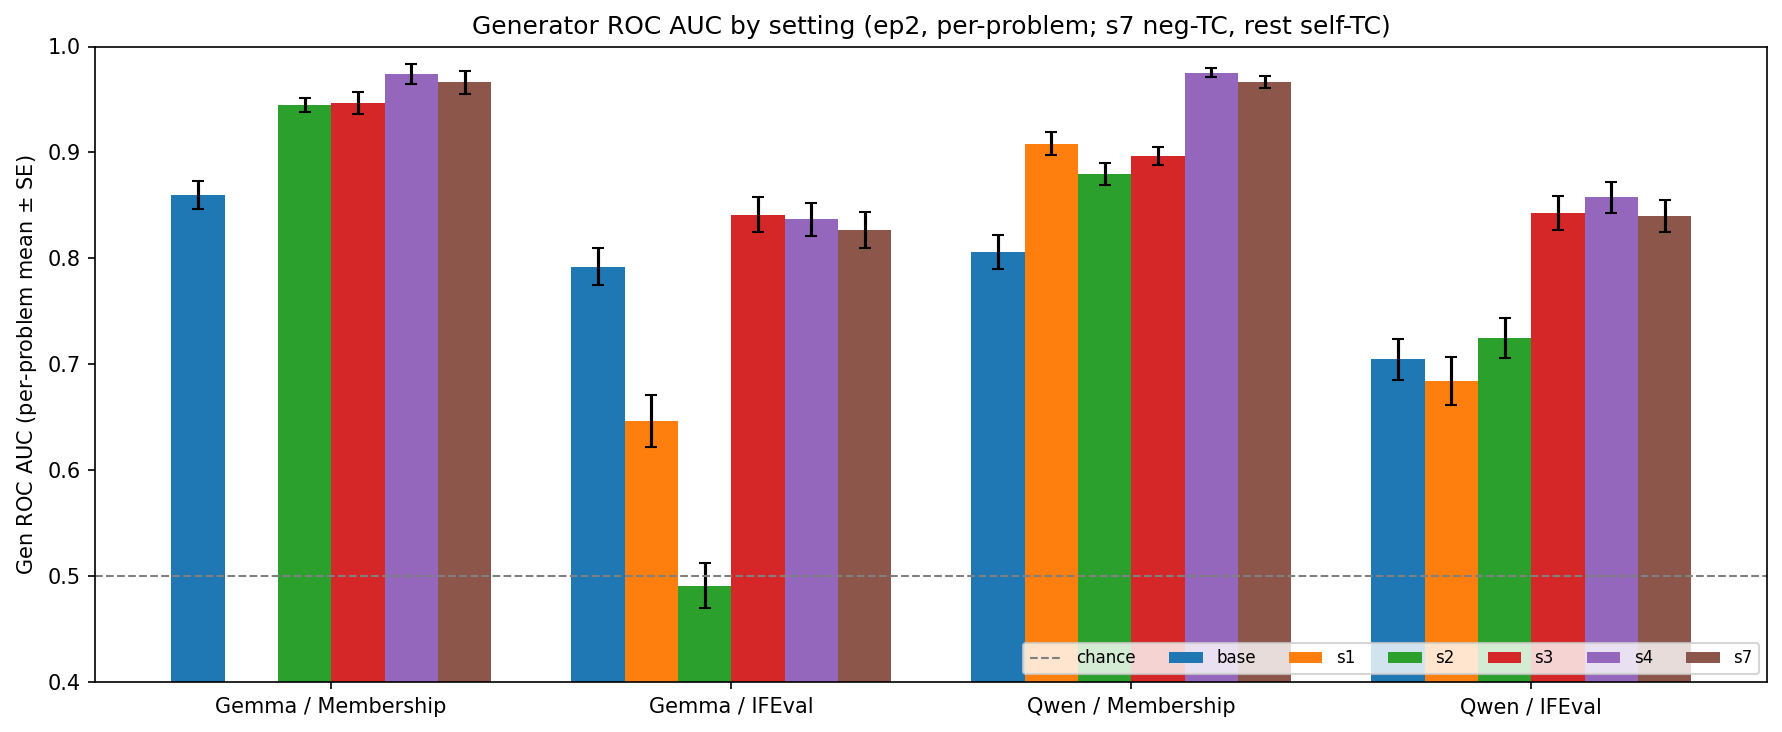
\includegraphics[width=0.95\textwidth]{plots/fix_unified_genroc.png}
\caption{Generator ROC AUC across settings and model/task combinations (epoch 2, train set),
\textbf{per-problem mean with SE error bars}. Self-TC scoring for all settings except s7 (neg-TC),
scored with neg-TC to match its training-time TC type. Dashed line is chance (0.5).}
\label{fig:unified_genroc}
\end{figure}

%% ============================================================
\section{Q2: Training Diagnostics}
%% ============================================================

\subsection{Loss Curves from WandB}

Training was monitored via WandB for gemma-ifeval, qwen-membership, and qwen-ifeval. Gemma-membership was trained before WandB logging was added.

\textbf{Smoothing.} All loss curves in this section are smoothed using a running average with a window of 20 steps. To replicate in WandB: open a line plot panel's settings $\to$ Data tab $\to$ Smoothing Type: ``Running Average'' $\to$ Smoothing Parameter: 20. Raw (unsmoothed) curves are available directly on WandB.

\subsubsection{IFEval}

\begin{figure}[H]
\centering
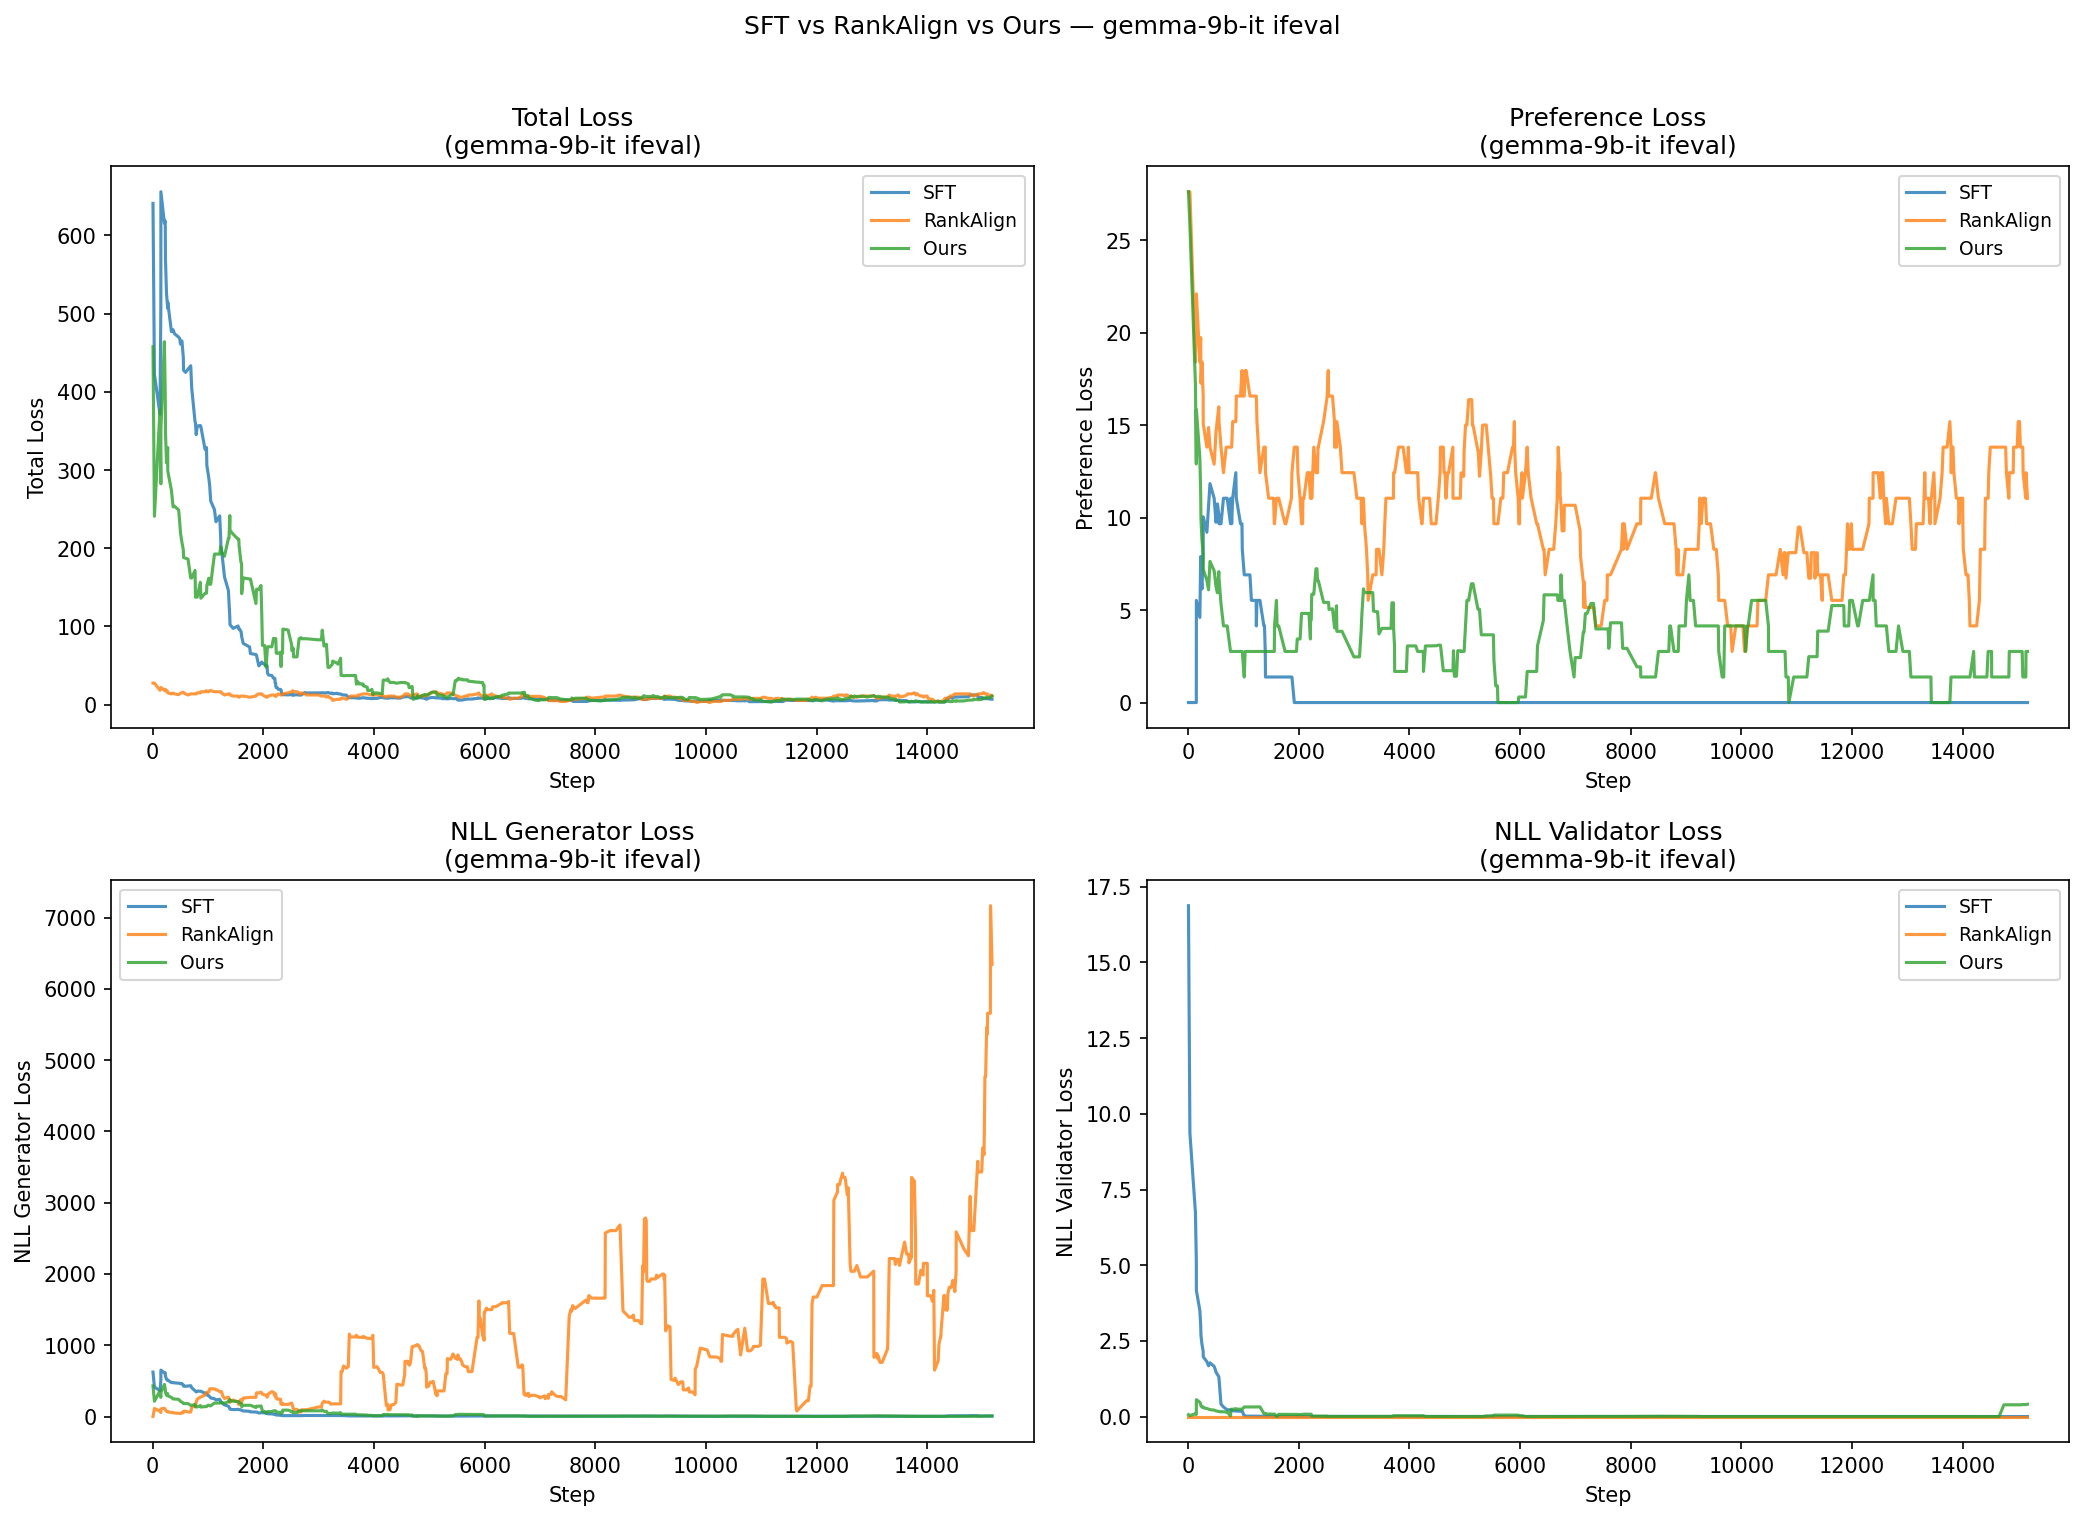
\includegraphics[width=0.95\textwidth]{plots/wandb_loss_methods_gemma-9b-it_ifeval.png}
\caption{Loss curves: SFT vs RankAlign vs Ours (gemma-2-9b-it, IFEval).}
\label{fig:loss_methods_gemma_ifeval}
\end{figure}

\begin{figure}[H]
\centering
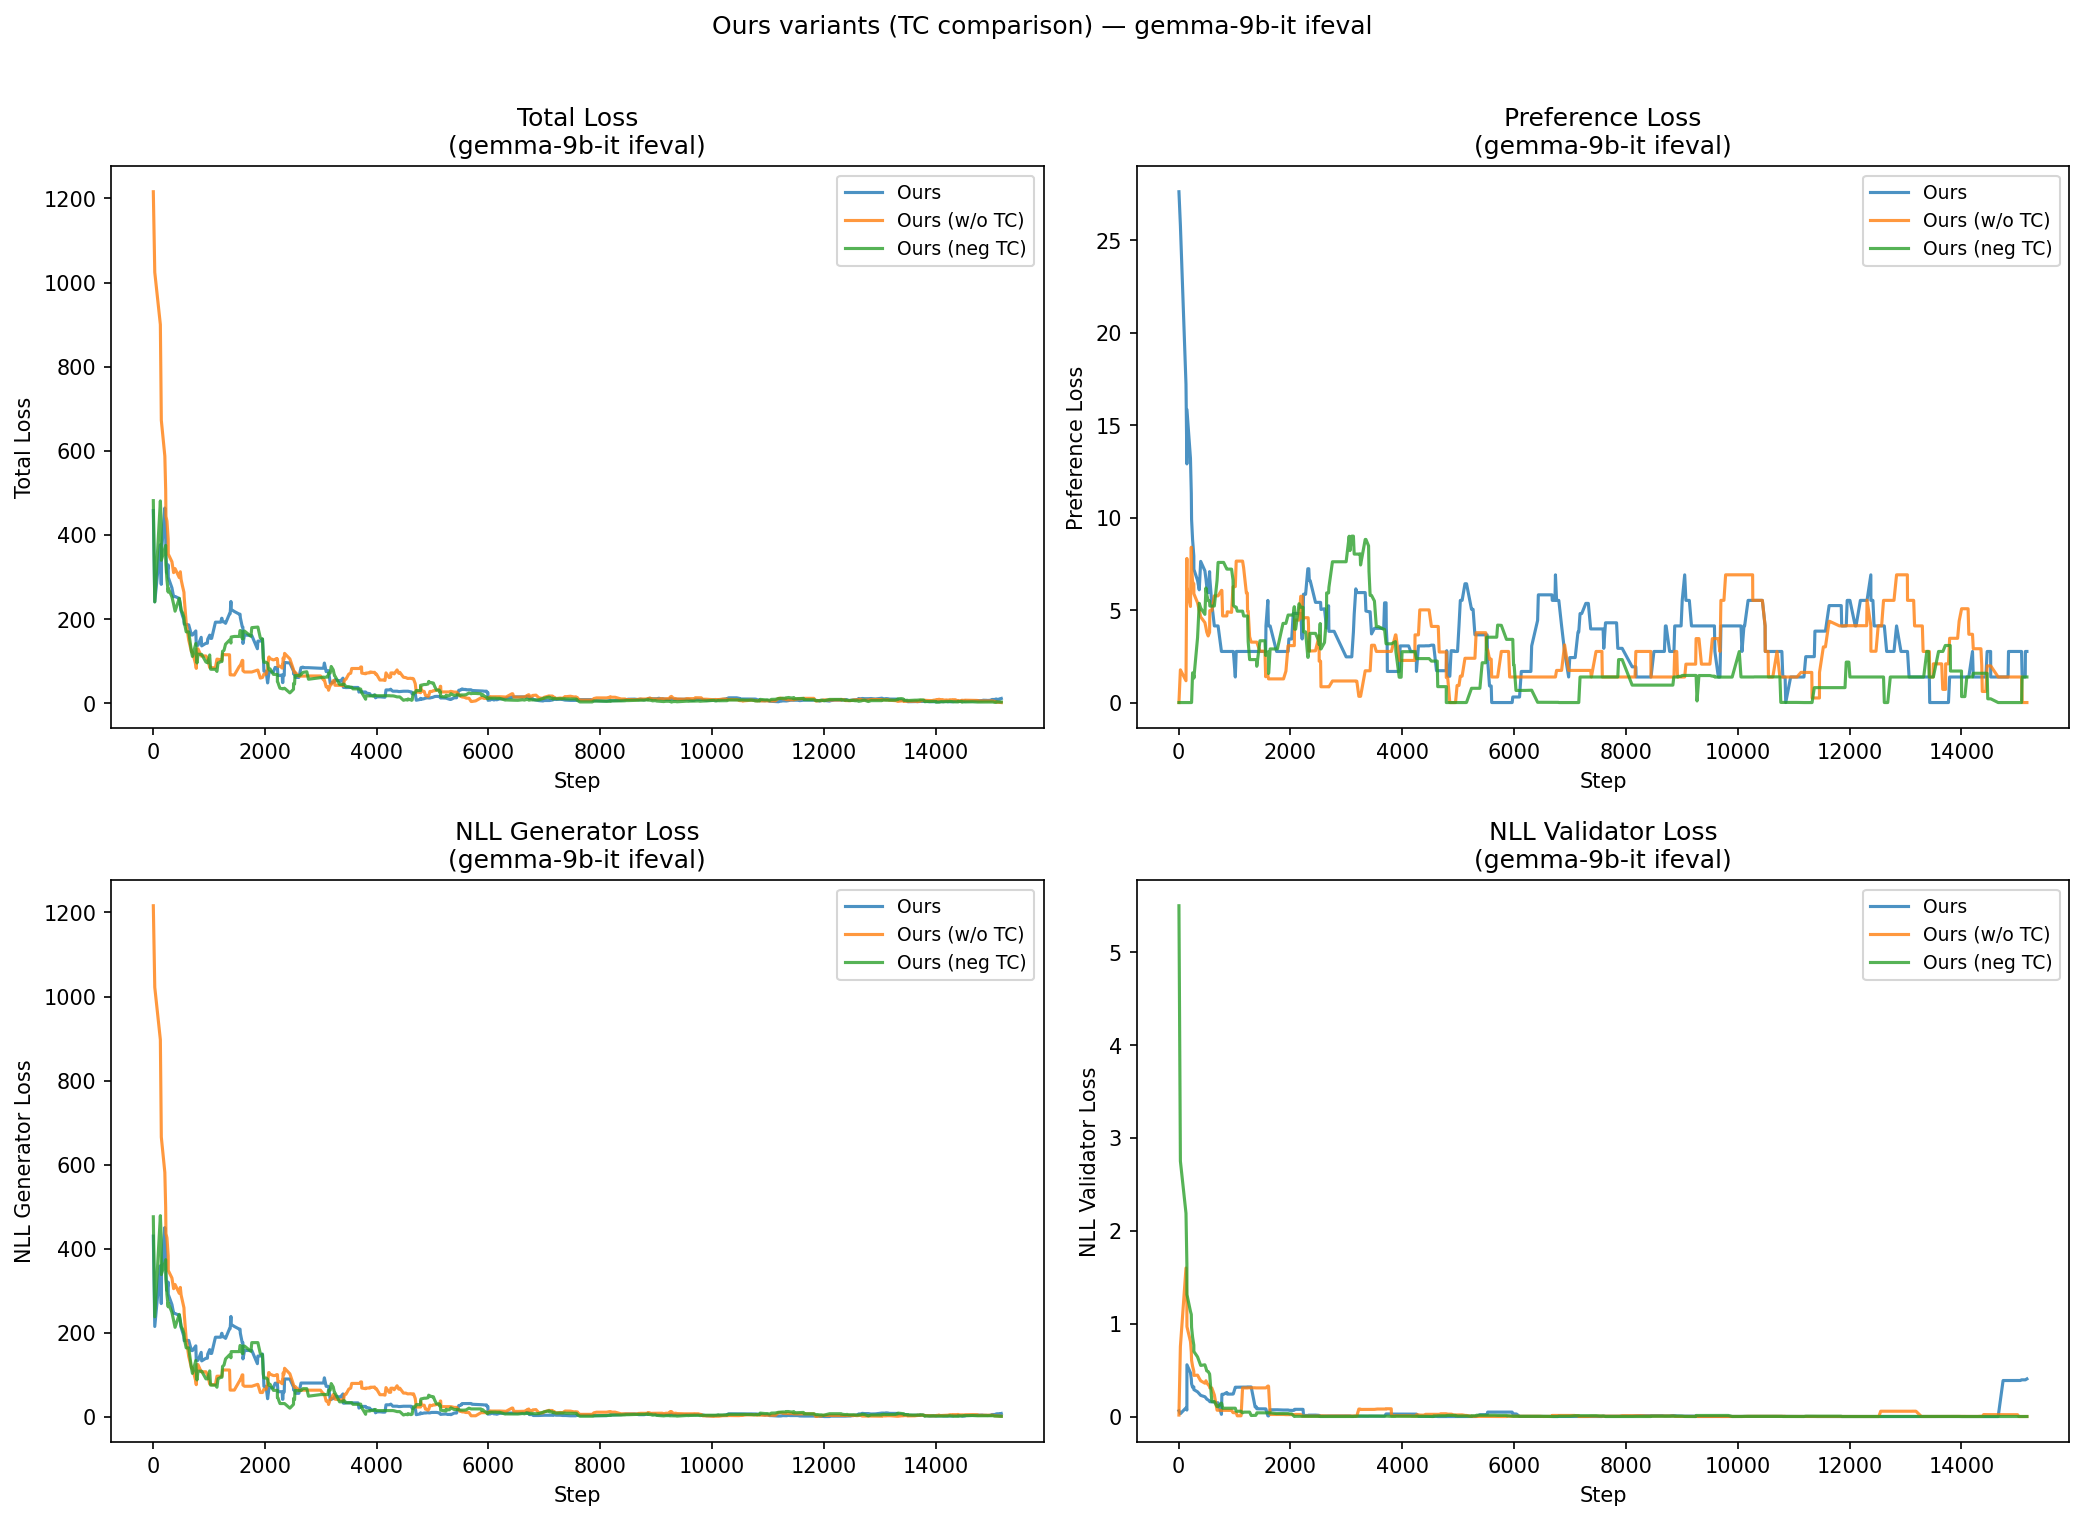
\includegraphics[width=0.95\textwidth]{plots/wandb_loss_tc_gemma-9b-it_ifeval.png}
\caption{Loss curves: Ours TC comparison (gemma-2-9b-it, IFEval).}
\label{fig:loss_tc_gemma_ifeval}
\end{figure}

\begin{figure}[H]
\centering

\includegraphics[width=0.95\textwidth]{{plots/wandb_loss_methods_qwen3.5-9b_ifeval}.png}
\caption{Loss curves: SFT vs RankAlign vs Ours (Qwen3.5-9B, IFEval).}
\label{fig:loss_methods_qwen_ifeval}
\end{figure}

\begin{figure}[H]
\centering

\includegraphics[width=0.95\textwidth]{{plots/wandb_loss_tc_qwen3.5-9b_ifeval}.png}
\caption{Loss curves: Ours TC comparison (Qwen3.5-9B, IFEval).}
\label{fig:loss_tc_qwen_ifeval}
\end{figure}

\subsubsection{Membership}

\emph{Note: gemma-2-9b-it membership was trained before WandB logging was added; no loss curves are available for that combination.}

\begin{figure}[H]
\centering

\includegraphics[width=0.95\textwidth]{{plots/wandb_loss_methods_qwen3.5-9b_membership}.png}
\caption{Loss curves: SFT vs RankAlign vs Ours (Qwen3.5-9B, membership).}
\label{fig:loss_methods_qwen_mem}
\end{figure}

\begin{figure}[H]
\centering

\includegraphics[width=0.95\textwidth]{{plots/wandb_loss_tc_qwen3.5-9b_membership}.png}
\caption{Loss curves: Ours TC comparison (Qwen3.5-9B, membership).}
\label{fig:loss_tc_qwen_mem}
\end{figure}

\subsection{Loss Component Breakdown}

Table~\ref{tab:loss_breakdown} reveals the root cause of s2's failure on IFEval: without an NLL-G constraint, the generator's NLL explodes to \textbf{3120} (vs.\ 3.8--4.3 for constrained settings).

\begin{table}[H]
\centering
\caption{Final-third loss components (Gemma IFEval). s2's NLL-G explosion explains its poor gen\_roc.}
\label{tab:loss_breakdown}
\begin{tabular}{lrrrr}
\toprule
\textbf{Setting} & \textbf{Total} & \textbf{Pref} & \textbf{NLL-G} & \textbf{NLL-V} \\
\midrule
s1 (SFT) & 5.99 & 0.00 & 5.99 & 0.000 \\
\textbf{s2 (basic)} & \textbf{11.56} & \textbf{11.56} & \textbf{3119.8} & 0.000 \\
s4 (TC-self) & 6.40 & 2.64 & 3.76 & 0.001 \\
s3 (full) & 6.15 & 1.81 & 4.33 & 0.009 \\
s7 (TC-neg) & 5.13 & 1.37 & 3.77 & 0.001 \\
\bottomrule
\end{tabular}
\end{table}

\textbf{Key insight}: On the simpler membership task (Qwen), s2 keeps NLL-G reasonable (2.42) without explicit constraint. The constraint is only critical for complex tasks where the optimization landscape allows score explosion.

\begin{figure}[H]
\centering
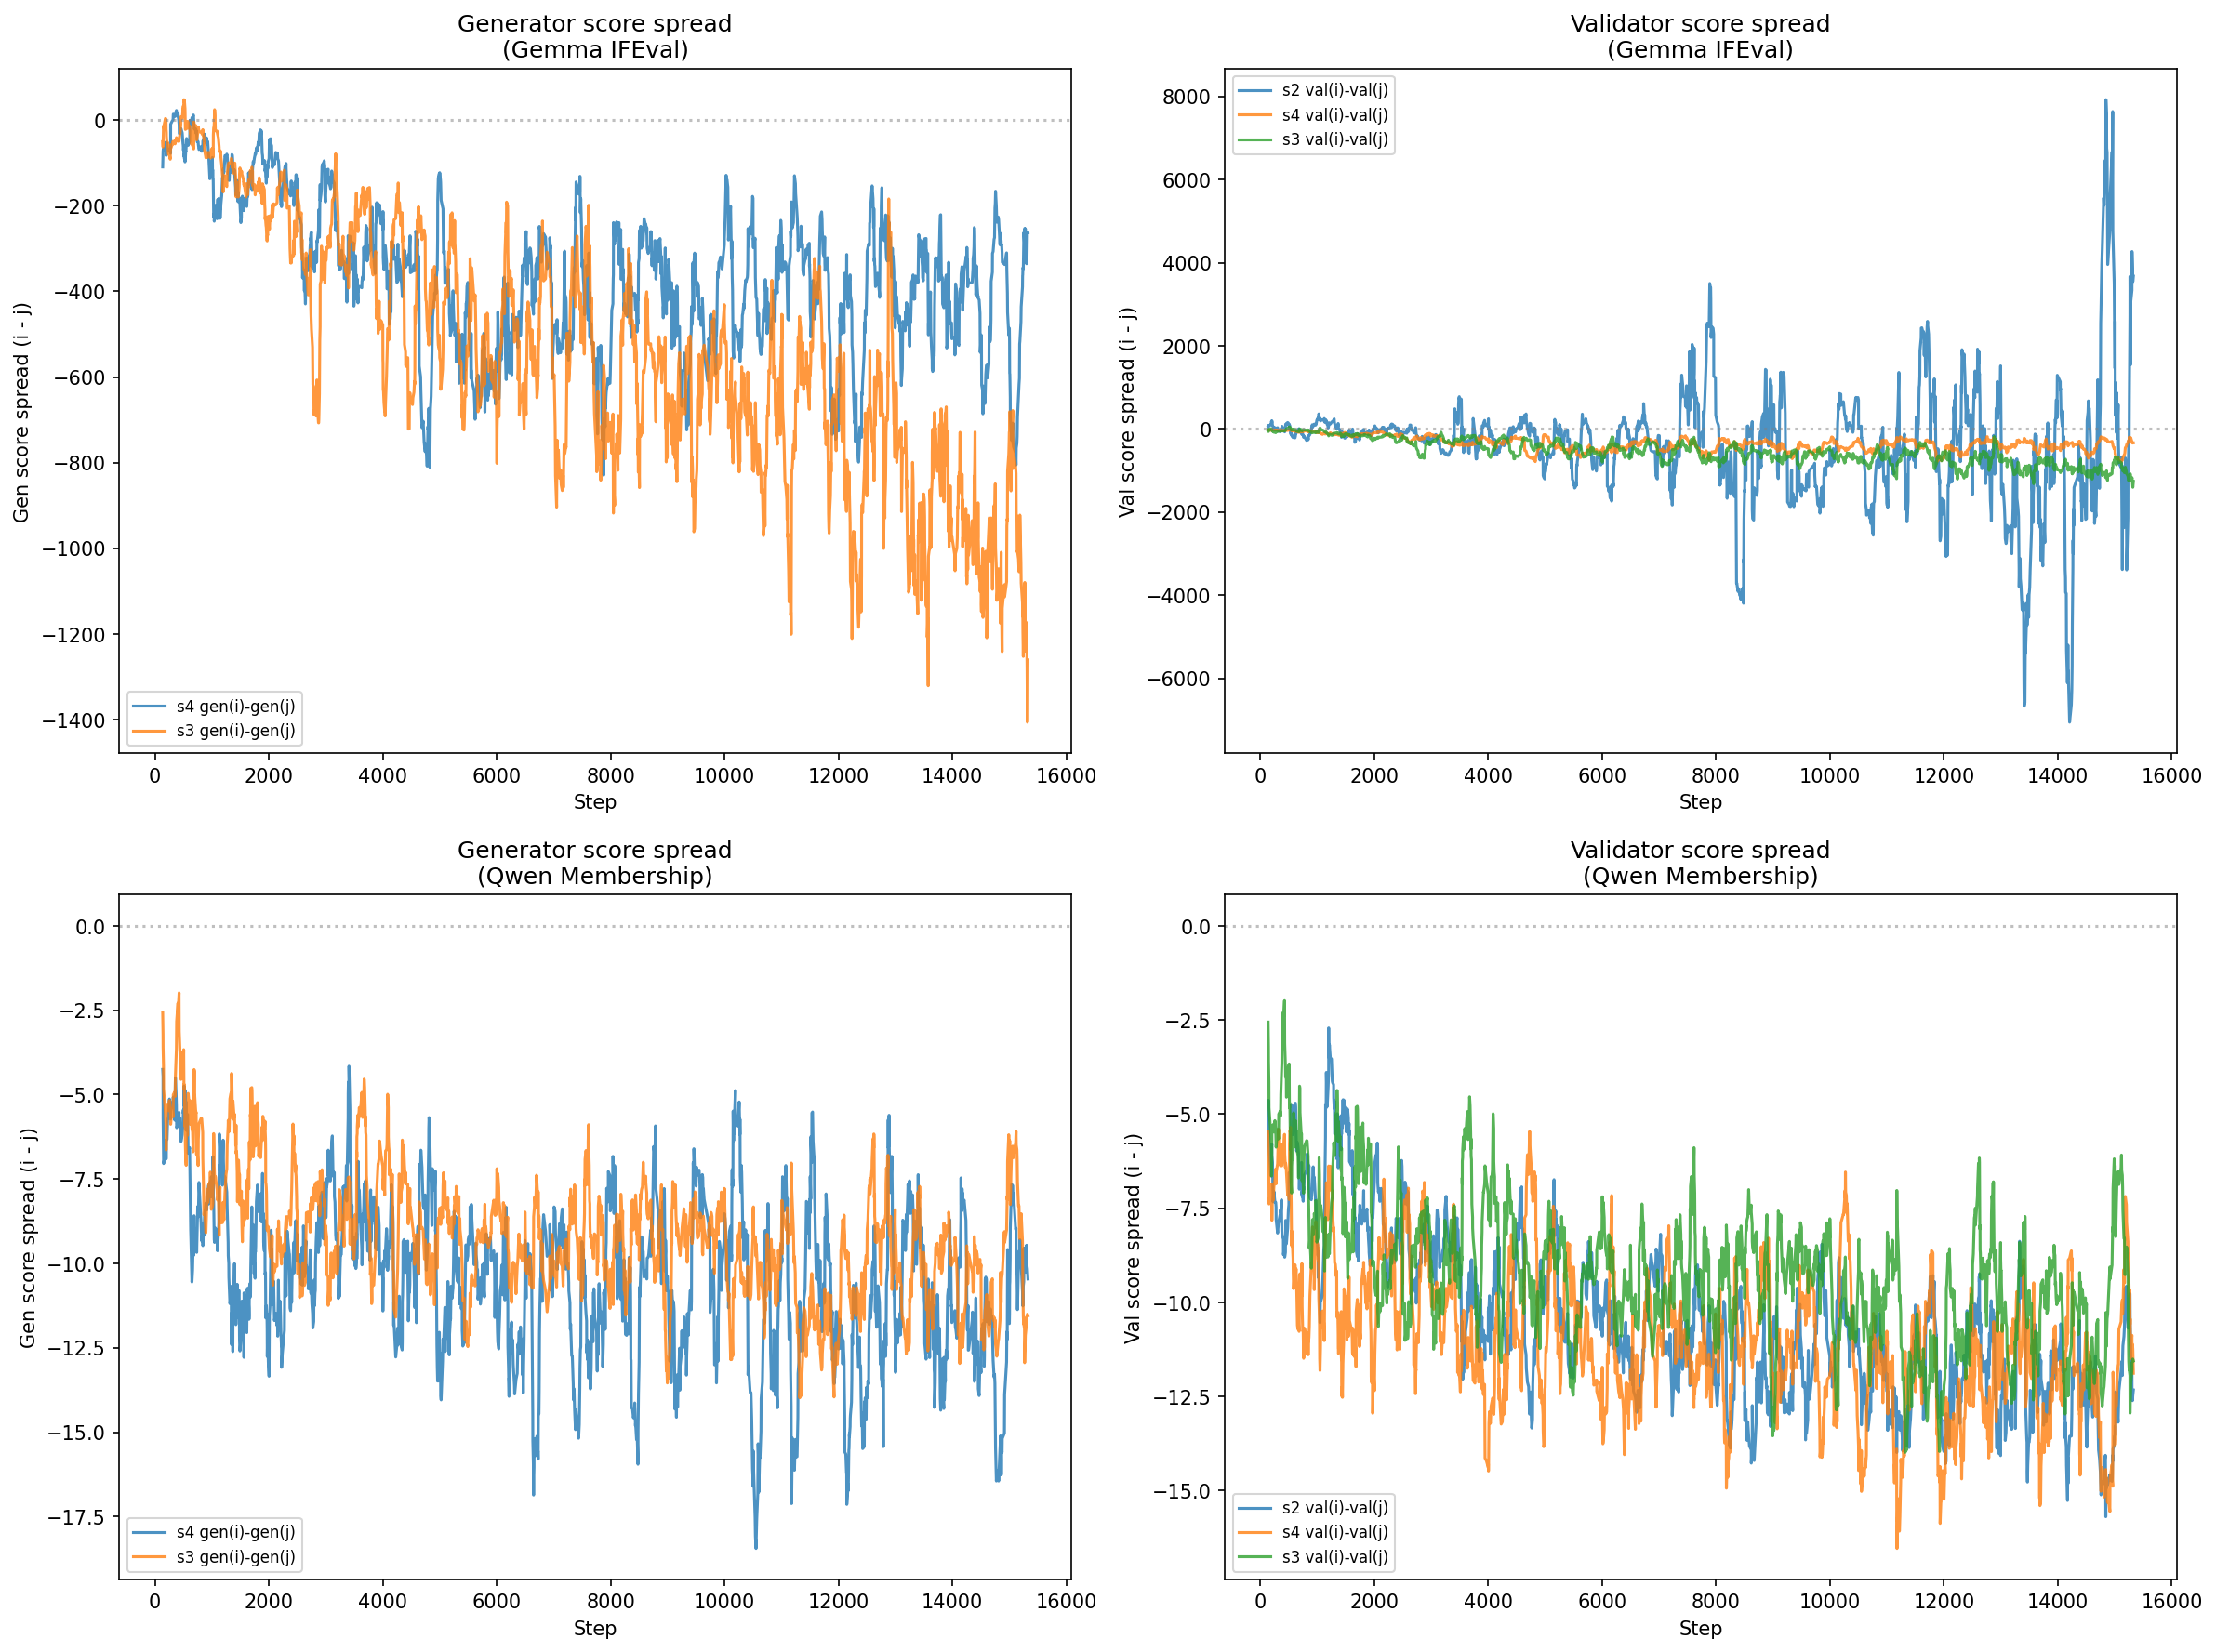
\includegraphics[width=0.95\textwidth]{plots/wandb_score_evolution.png}
\caption{Score spread evolution during training. Each curve plots the difference between the two scores in a sampled training pair (item $i$ minus item $j$) at each logged step, smoothed with a 20-step running average. Generator panels (left column) include only settings with $\text{NLL}_G > 0$ (s2 with $\text{NLL}_G=0$ does not log per-item generator scores), so only s3 and s4 appear there; validator panels (right column) include s2, s3, s4. A more negative spread indicates a wider learned margin between the two paired items.}
\label{fig:score_evolution}
\end{figure}

\subsection{Held-out Validation Loss}

The WandB curves above are training-set losses. To check whether each setting also reduces loss on \emph{held-out} data, we recompute the same three loss components (preference, NLL-G, NLL-V) on a test set for each checkpoint (base, epoch 0, 1, 2). The base row is identical across settings (same untrained \texttt{gemma-2-9b-it}) and is shown as a dashed reference line in each panel.

\textbf{Test sets.}
\begin{itemize}
\item \emph{Gemma / IFEval}: the held-out 50\% of \texttt{ifeval-concat} (4{,}760 test items: 2{,}223 positive, 2{,}537 negative). 500 (positive, negative) pairs are sampled with a fixed seed.
\item \emph{Gemma / Membership}: \texttt{membership-sans-rosch-v0} is trained \emph{without} rosch, so its held-out distribution is rosch itself. We aggregate \texttt{L\_test} across all 11 registered \texttt{rosch-*} per-category tasks (1{,}042 items: 521 positive, 521 negative) and again sample 500 pairs.
\end{itemize}

The losses are computed with the same definitions used at training time: preference loss uses gen-score margins between the positive and negative item, NLL-G is the negative log-likelihood of the generator's gold completion, and NLL-V is the negative log-likelihood of the discriminator's correct yes/no token. Pairs and prompts are constructed by the same \texttt{make\_prompt} the training script uses (membership models are evaluated under rosch's prompt template, which uses the same \emph{``Complete the sentence: an example of \dots''} family as membership).

\begin{figure}[H]
\centering
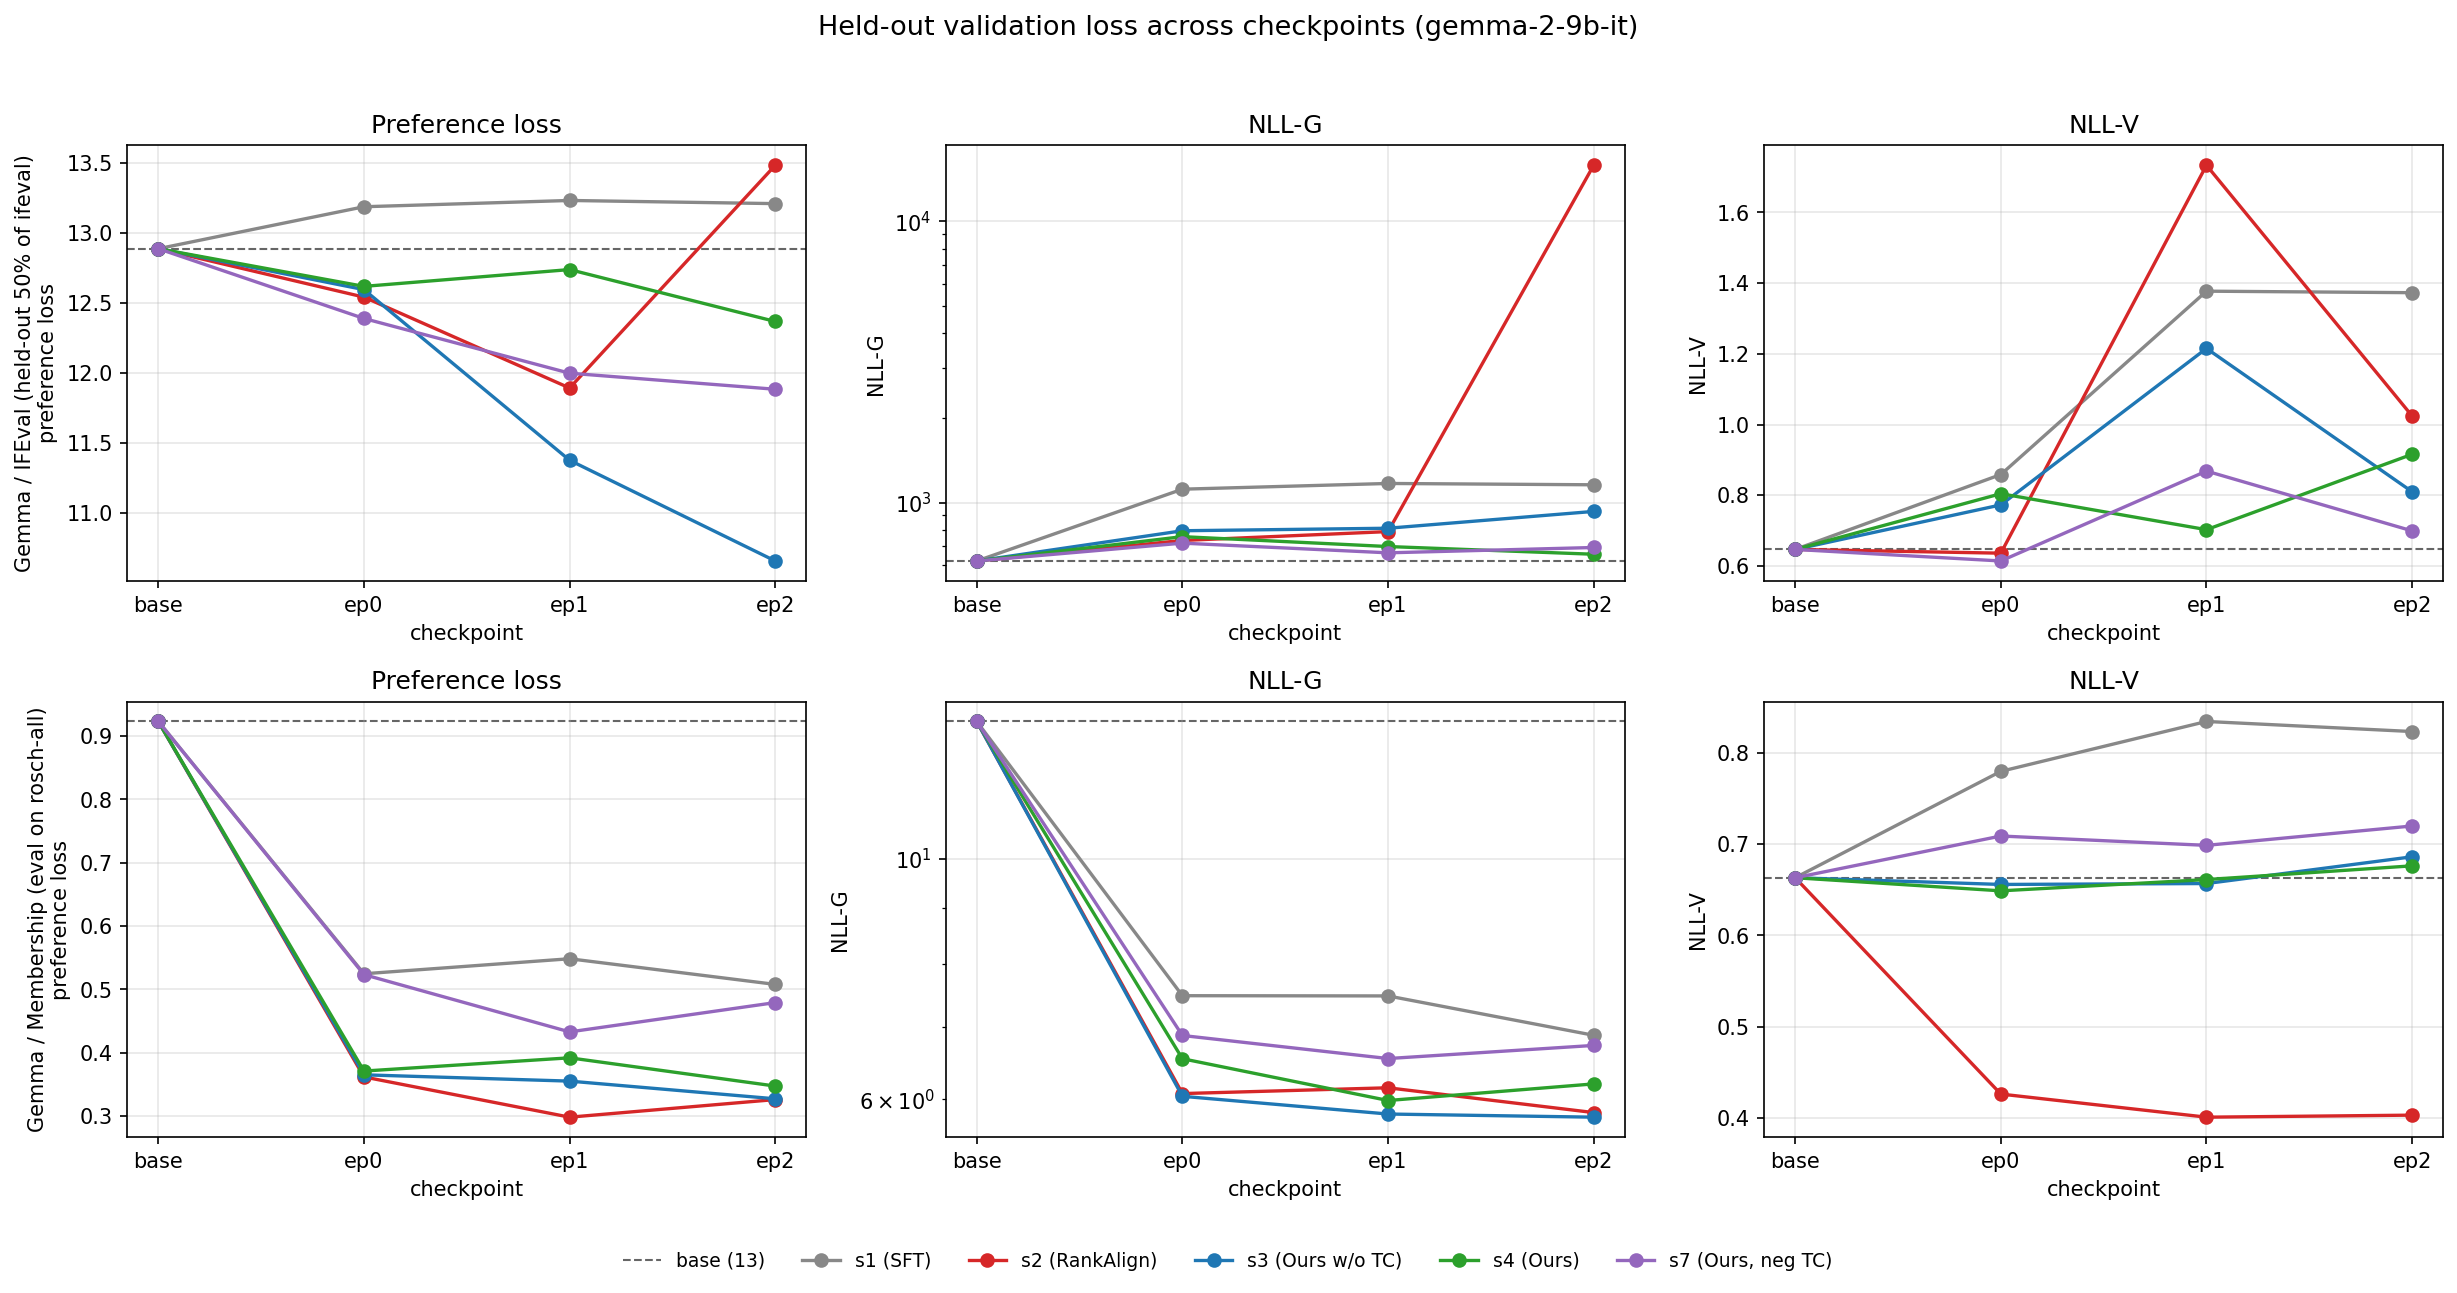
\includegraphics[width=0.95\textwidth]{plots/val_loss_curves.png}
\caption{Held-out validation loss across checkpoints for gemma-2-9b-it. Top row: IFEval (held-out 50\%). Bottom row: membership models evaluated on the aggregated rosch test set. The NLL-G column uses a log $y$-axis because s2 IFEval diverges. Dashed black line is the untrained base; markers at \texttt{ep0/ep1/ep2} show the three saved checkpoints from each setting.}
\label{fig:val_loss}
\end{figure}

\textbf{Reading the figure.}
\begin{itemize}
\item On membership/rosch (bottom row), every setting reduces all three losses substantially below base, and the orderings broadly match the train-set ranking (s3 and s2 lowest NLL-G; s4 and s3 lowest preference loss). This is the regime where RankAlign generalizes cleanly.
\item On IFEval (top row), the picture is much harder. Preference loss only drops materially for s3 ($12.89 \to 10.66$); s1 and s2 \emph{rise} above base. The NLL-G panel is the headline: s2's generator NLL explodes to roughly $1.6\times10^4$ by epoch 2 on held-out IFEval, mirroring the train-side observation reported in Section~2.2. The constrained settings (s4, s3, s7) keep NLL-G in the same order of magnitude as base and are the only ones whose held-out preference loss does not regress.
\item NLL-V tells a related story: s2 spikes the validator NLL on IFEval at epoch 1 before partially recovering, consistent with the score-explosion diagnostic --- the validator becomes badly miscalibrated before it can re-stabilize. On membership, by contrast, s2 drives NLL-V down most aggressively (the validator becomes very confident there).
\end{itemize}

This held-out view confirms what the train-side curves and the Q1 ROC numbers already imply: \emph{basic RankAlign without NLL constraints (s2) is unsafe on the harder IFEval task, even on data drawn from the same distribution} --- it is not just an in-sample optimization artifact.

\paragraph{Reproducibility.} The full pipeline lives at commit \texttt{3b71d4ac} on branch \texttt{longform}. Files involved:

\begin{itemize}
\item \textbf{Compute (Python)}: \texttt{scripts/compute\_val\_loss.py}. Loads the base model from \texttt{--model} plus the three merged epoch checkpoints found under \texttt{--models-dir} matching the \texttt{--setting} pattern; loads test data via \texttt{src/utils.py}'s \texttt{get\_task} (with \texttt{import tasks} side-effect to register all task modules). For each checkpoint it computes the same three loss components used at training time and writes one row per (setting, checkpoint) to the CSV at \texttt{--output} (appending). Defaults: \texttt{--max-pairs 500}, \texttt{--seed 42}.
\item \textbf{Special test-set logic for membership}: when \texttt{--test-task rosch-all} is passed, \texttt{compute\_val\_loss.py} aggregates \texttt{L\_test} across every registered \texttt{rosch-*} task (1{,}042 items) and uses rosch's \texttt{make\_prompt}/\texttt{get\_label} for prompt construction. For ifeval, no \texttt{--test-task} is needed --- the task itself returns a held-out split.
\item \textbf{Launcher (Slurm)}: \texttt{scripts/run\_val\_loss.sh}. Reads env vars \texttt{MODEL}, \texttt{TASK}, \texttt{TEST\_TASK}, \texttt{MODELS\_DIR}, \texttt{SETTINGS}, \texttt{OUTPUT}, \texttt{HOURS}, exports \texttt{HF\_HOME=/datastor2/jdr/.cache/huggingface} so all jobs reuse the existing \texttt{gemma-2-9b-it} snapshot (otherwise five concurrent jobs each redownload $\sim$36\,GB and blow the home-filer quota), then submits one Slurm job per setting via \texttt{\textasciitilde/.local/bin/run 1 \$HOURS --mem 64G ...}.
\item \textbf{Exact commands run} (from the repo root, \texttt{/datastor1/jdr/gv-gap/rankalign}, with \texttt{venv\_lexcons} activated):
\begin{verbatim}
# IFEval val-loss (5 jobs: 44826-44830, ~1h52m each on 1 GPU)
TASK=ifeval-concat \
OUTPUT=analysis/tables/val_loss_gemma_ifeval.csv \
bash scripts/run_val_loss.sh

# Membership val-loss, evaluated on rosch (5 jobs: 44831-44835, ~14m each)
TASK=membership-sans-rosch-v0 \
TEST_TASK=rosch-all \
OUTPUT=analysis/tables/val_loss_gemma_mem.csv \
bash scripts/run_val_loss.sh
\end{verbatim}
Both runs use the default \texttt{MODEL=google/gemma-2-9b-it}, \texttt{MODELS\_DIR=/datastor2/jdr/rankalign/models2-rerun-wandb}, and \texttt{SETTINGS="s1 s2 s3 s4 s7"}.
\item \textbf{Output CSVs} (one row per setting/checkpoint, columns: \texttt{checkpoint, setting, model, task, n\_pos, n\_neg, n\_pairs, preference\_loss, nll\_generator\_loss, nll\_validator\_loss, total\_loss, mean\_gen\_score\_pos, mean\_gen\_score\_neg, mean\_val\_score\_pos, mean\_val\_score\_neg}):
\begin{itemize}
\item \texttt{analysis/tables/val\_loss\_gemma\_ifeval.csv}
\item \texttt{analysis/tables/val\_loss\_gemma\_mem.csv}
\end{itemize}
\item \textbf{Plot (Python)}: \texttt{analysis/scripts/plot\_val\_loss.py}, run as
\begin{verbatim}
python analysis/scripts/plot_val_loss.py
\end{verbatim}
This reads the two CSVs above (paths hard-coded relative to repo root) and writes \texttt{analysis/plots/val\_loss\_curves.png}, the figure shown above. NLL-G uses a log $y$-axis; preference loss and NLL-V use linear.
\end{itemize}

\subsection{Generator-Validator Concordance}

Concordance measures the fraction of item pairs where the generator and validator agree on the ordering direction.

\begin{table}[H]
\centering
\caption{Concordance at epoch 2 (self-TC scoring), per-problem mean$\pm$SE. Chance = 0.5.}
\label{tab:concordance}
% Auto-generated by build_report_fix_metrics.py. metric=concordance
\begin{tabular}{lccccc}
\toprule
\textbf{Model / Task} & \textbf{Base} & \textbf{s1} & \textbf{s2} & \textbf{s3} & \textbf{s4} \\
\midrule
Gemma / Membership & $0.716\se{0.010}$ & --- & $0.785\se{0.006}$ & $0.805\se{0.005}$ & $\mathbf{0.826}\se{0.006}$ \\
Gemma / IFEval & $0.654\se{0.010}$ & $0.598\se{0.013}$ & $0.460\se{0.013}$ & $0.748\se{0.009}$ & $\mathbf{0.757}\se{0.007}$ \\
Qwen / Membership & $0.680\se{0.009}$ & $0.740\se{0.007}$ & $0.753\se{0.006}$ & $0.768\se{0.005}$ & $\mathbf{0.835}\se{0.005}$ \\
Qwen / IFEval & $0.600\se{0.012}$ & $0.594\se{0.012}$ & $0.596\se{0.010}$ & $0.742\se{0.008}$ & $\mathbf{0.750}\se{0.008}$ \\
\bottomrule
\end{tabular}

\end{table}

Note: s2 on Gemma IFEval has per-problem concordance $0.460$ (below the 0.5 chance line); the
anti-correlation between generator and validator is clearer in the per-problem Spearman, where s2
on Gemma/IFEval is negative ($-0.113\se{0.037}$).

\subsection{Spearman Correlation (Generator vs Validator)}

\begin{table}[H]
\centering
\caption{Spearman $\rho$ between generator and validator scores (epoch 2, self-TC), per-problem
mean$\pm$SE.}
\label{tab:spearman}
% Auto-generated by build_report_fix_metrics.py. metric=spearman
\begin{tabular}{lccccc}
\toprule
\textbf{Model / Task} & \textbf{Base} & \textbf{s1} & \textbf{s2} & \textbf{s3} & \textbf{s4} \\
\midrule
Gemma / Membership & $0.595\se{0.024}$ & --- & $0.763\se{0.014}$ & $0.803\se{0.011}$ & $\mathbf{0.839}\se{0.008}$ \\
Gemma / IFEval & $0.439\se{0.026}$ & $0.282\se{0.036}$ & $-0.113\se{0.037}$ & $0.670\se{0.021}$ & $\mathbf{0.697}\se{0.015}$ \\
Qwen / Membership & $0.508\se{0.024}$ & $0.668\se{0.017}$ & $0.687\se{0.014}$ & $0.725\se{0.011}$ & $\mathbf{0.855}\se{0.007}$ \\
Qwen / IFEval & $0.290\se{0.033}$ & $0.273\se{0.035}$ & $0.272\se{0.029}$ & $0.661\se{0.020}$ & $\mathbf{0.680}\se{0.018}$ \\
\bottomrule
\end{tabular}

\end{table}

\subsection{Pearson Correlation (Generator vs Validator)}

\begin{table}[H]
\centering
\caption{Pearson $r$ between generator and validator scores (epoch 2, self-TC), per-problem
mean$\pm$SE.}
\label{tab:pearson}
% Auto-generated by build_report_fix_metrics.py. metric=pearson
\begin{tabular}{lccccc}
\toprule
\textbf{Model / Task} & \textbf{Base} & \textbf{s1} & \textbf{s2} & \textbf{s3} & \textbf{s4} \\
\midrule
Gemma / Membership & $0.594\se{0.022}$ & --- & $0.802\se{0.014}$ & $0.827\se{0.011}$ & $\mathbf{0.897}\se{0.006}$ \\
Gemma / IFEval & $0.453\se{0.030}$ & $0.271\se{0.041}$ & $-0.107\se{0.038}$ & $\mathbf{0.762}\se{0.022}$ & $0.736\se{0.016}$ \\
Qwen / Membership & $0.538\se{0.023}$ & $0.702\se{0.017}$ & $0.716\se{0.014}$ & $0.739\se{0.011}$ & $\mathbf{0.876}\se{0.004}$ \\
Qwen / IFEval & $0.297\se{0.034}$ & $0.291\se{0.037}$ & $0.280\se{0.032}$ & $\mathbf{0.765}\se{0.021}$ & $0.706\se{0.019}$ \\
\bottomrule
\end{tabular}

\end{table}

Pearson tracks Spearman on the membership tasks (s4 highest). On the IFEval tasks, s3 has higher Pearson than s4 even though s4 has higher Spearman --- s4 preserves rank order while compressing absolute magnitudes via TC.

\subsection{Score Delta Distributions}

\begin{figure}[H]
\centering
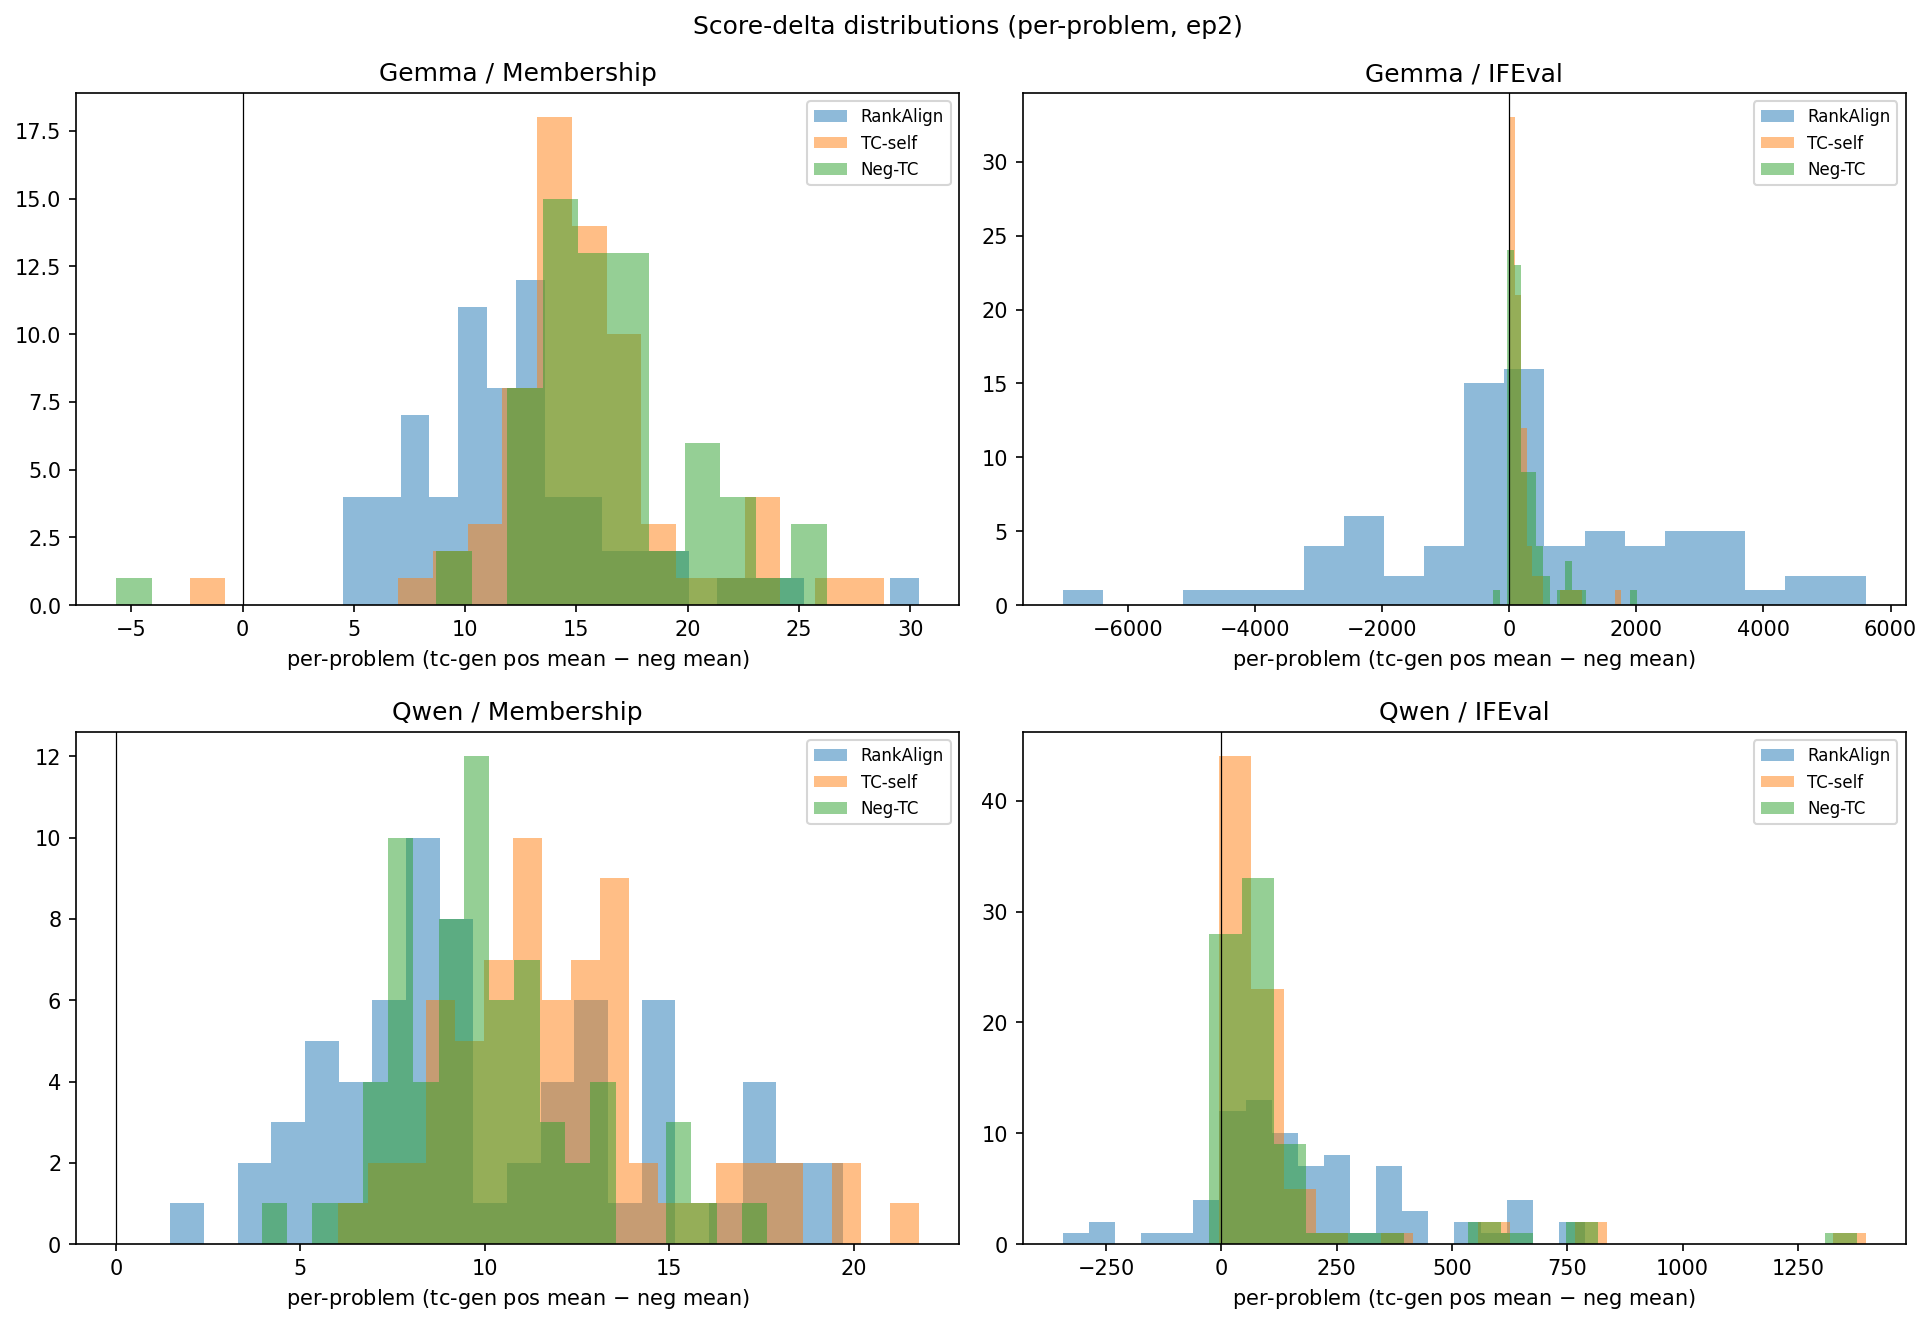
\includegraphics[width=0.95\textwidth]{plots/fix_score_delta_hist.png}
\caption{Per-problem score-delta distributions (ep2): one value per problem $=$ mean
typicality-corrected generator score of correct candidates minus that of incorrect candidates,
histogrammed over problems (s2/s4/s7). Mass above 0 means correct candidates score higher within
the problem. Same procedure as the HumanEval report.}
\label{fig:delta_histograms}
\end{figure}

\subsection{Training Dynamics}

\begin{figure}[H]
\centering
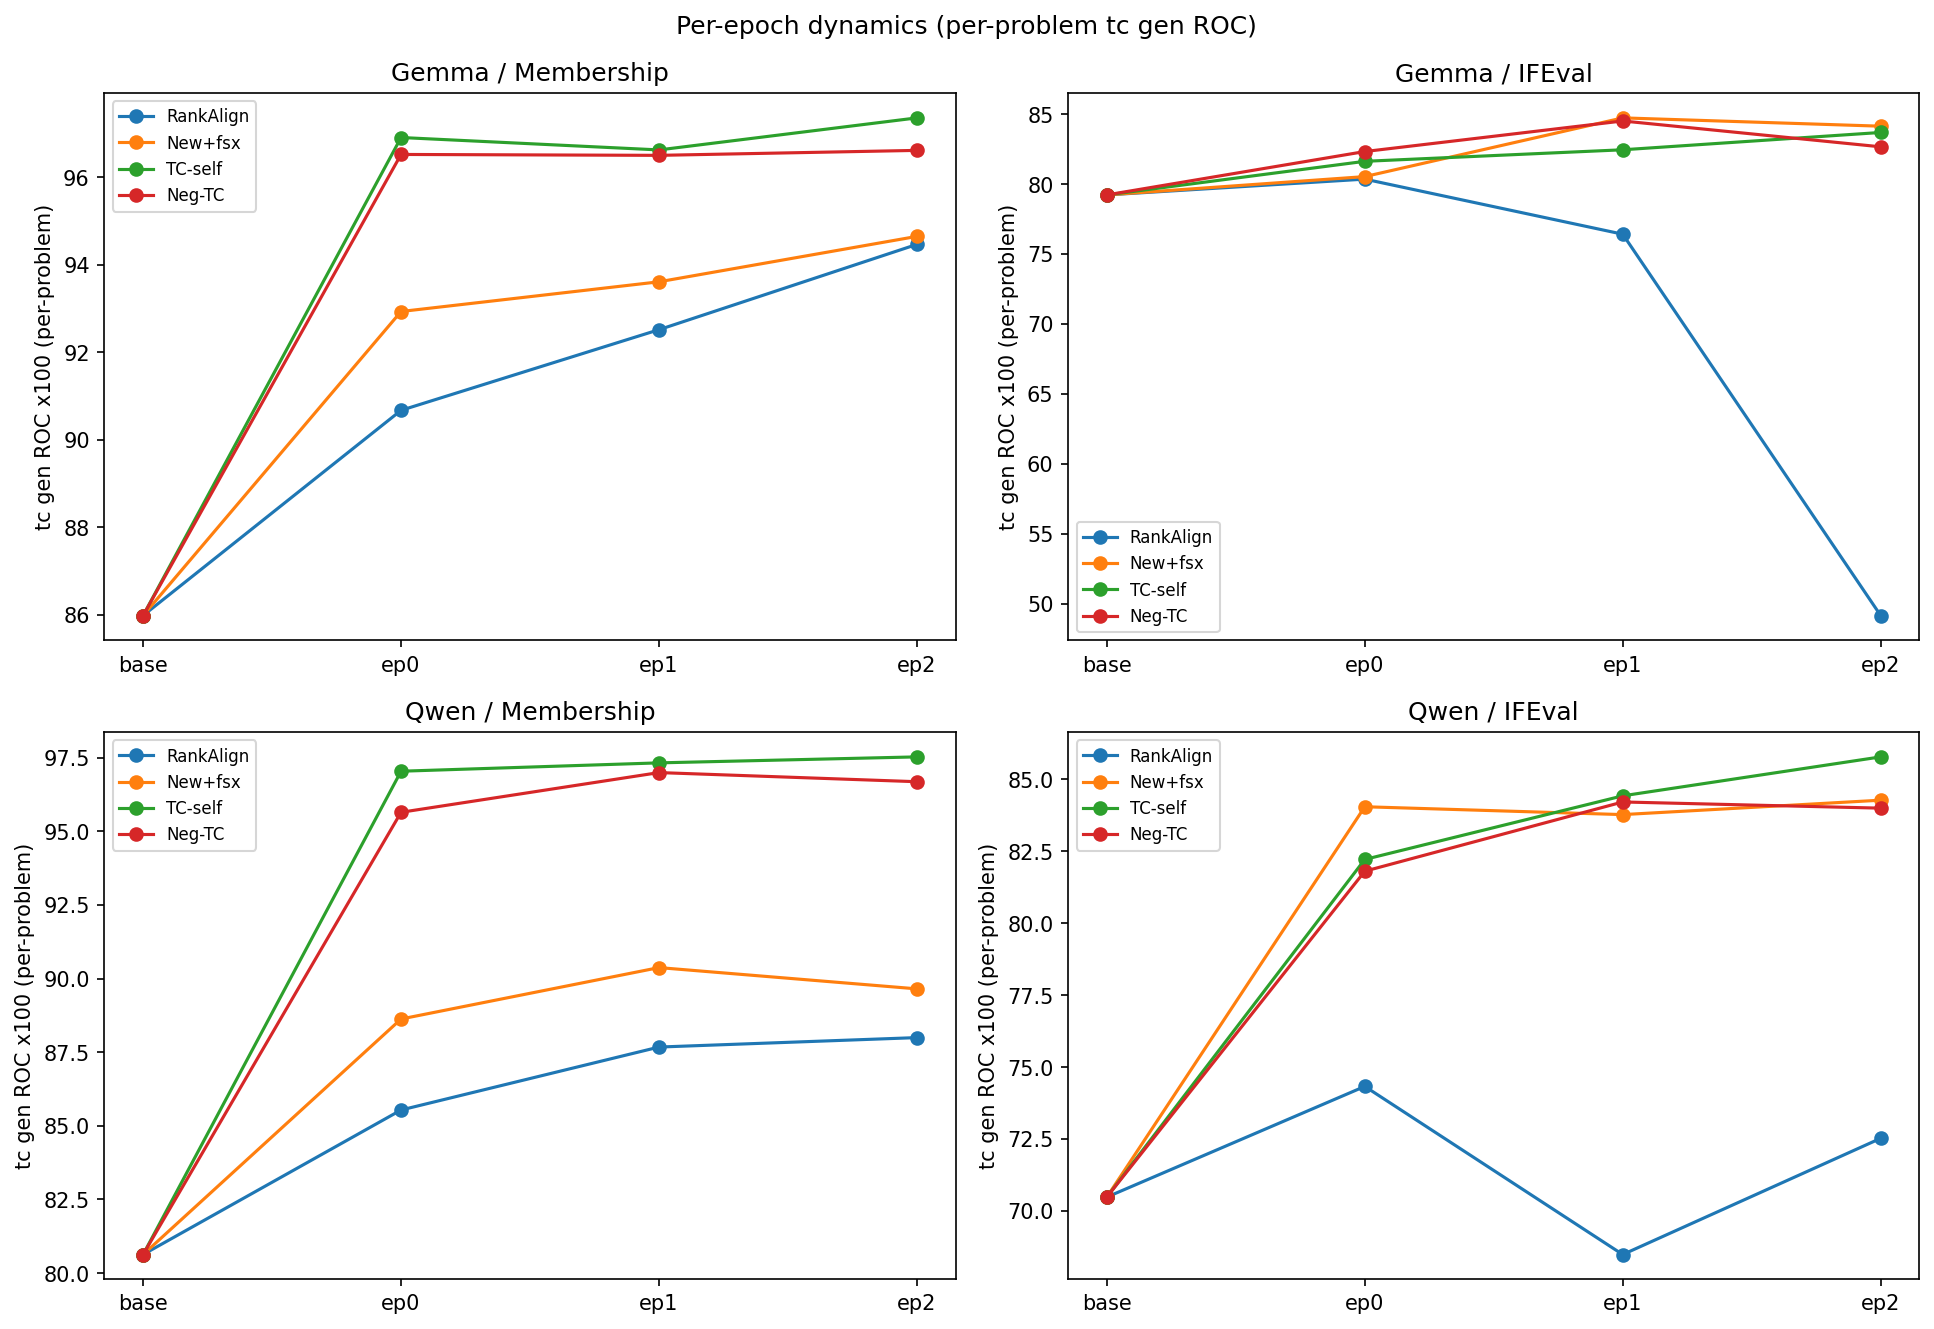
\includegraphics[width=0.95\textwidth]{plots/fix_tc_dynamics.png}
\caption{Per-epoch training dynamics: per-problem typicality-corrected gen ROC ($\times100$) vs.\
checkpoint (base/ep0/ep1/ep2) for s2/s3/s4/s7, each in its natural eval mode, across all four
model/task cells. Same per-problem procedure as the HumanEval report. Note RankAlign (s2) on
Gemma/IFEval collapses toward chance by ep2.}
\label{fig:dynamics}
\end{figure}

\begin{figure}[H]
\centering
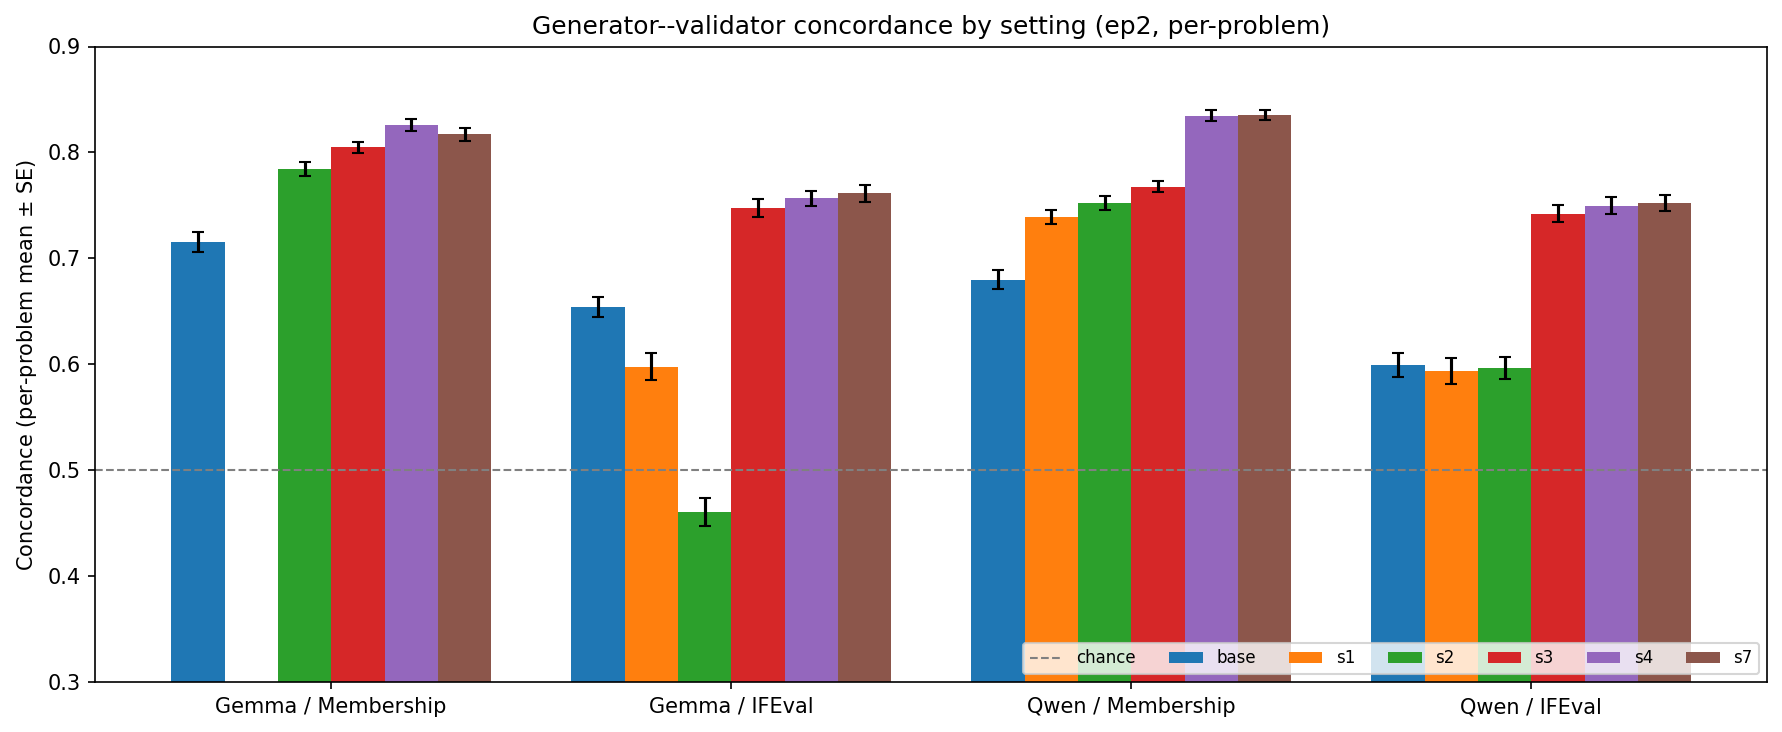
\includegraphics[width=0.95\textwidth]{plots/fix_unified_concordance.png}
\caption{Generator--validator concordance by setting (ep2), \textbf{per-problem mean with SE error
bars}, across all four cells. Dashed line is chance (0.5); s2 on Gemma/IFEval falls below it.}
\label{fig:concordance}
\end{figure}

\subsection{Generator-Validator Scatter Plots}

\begin{figure}[H]
\centering
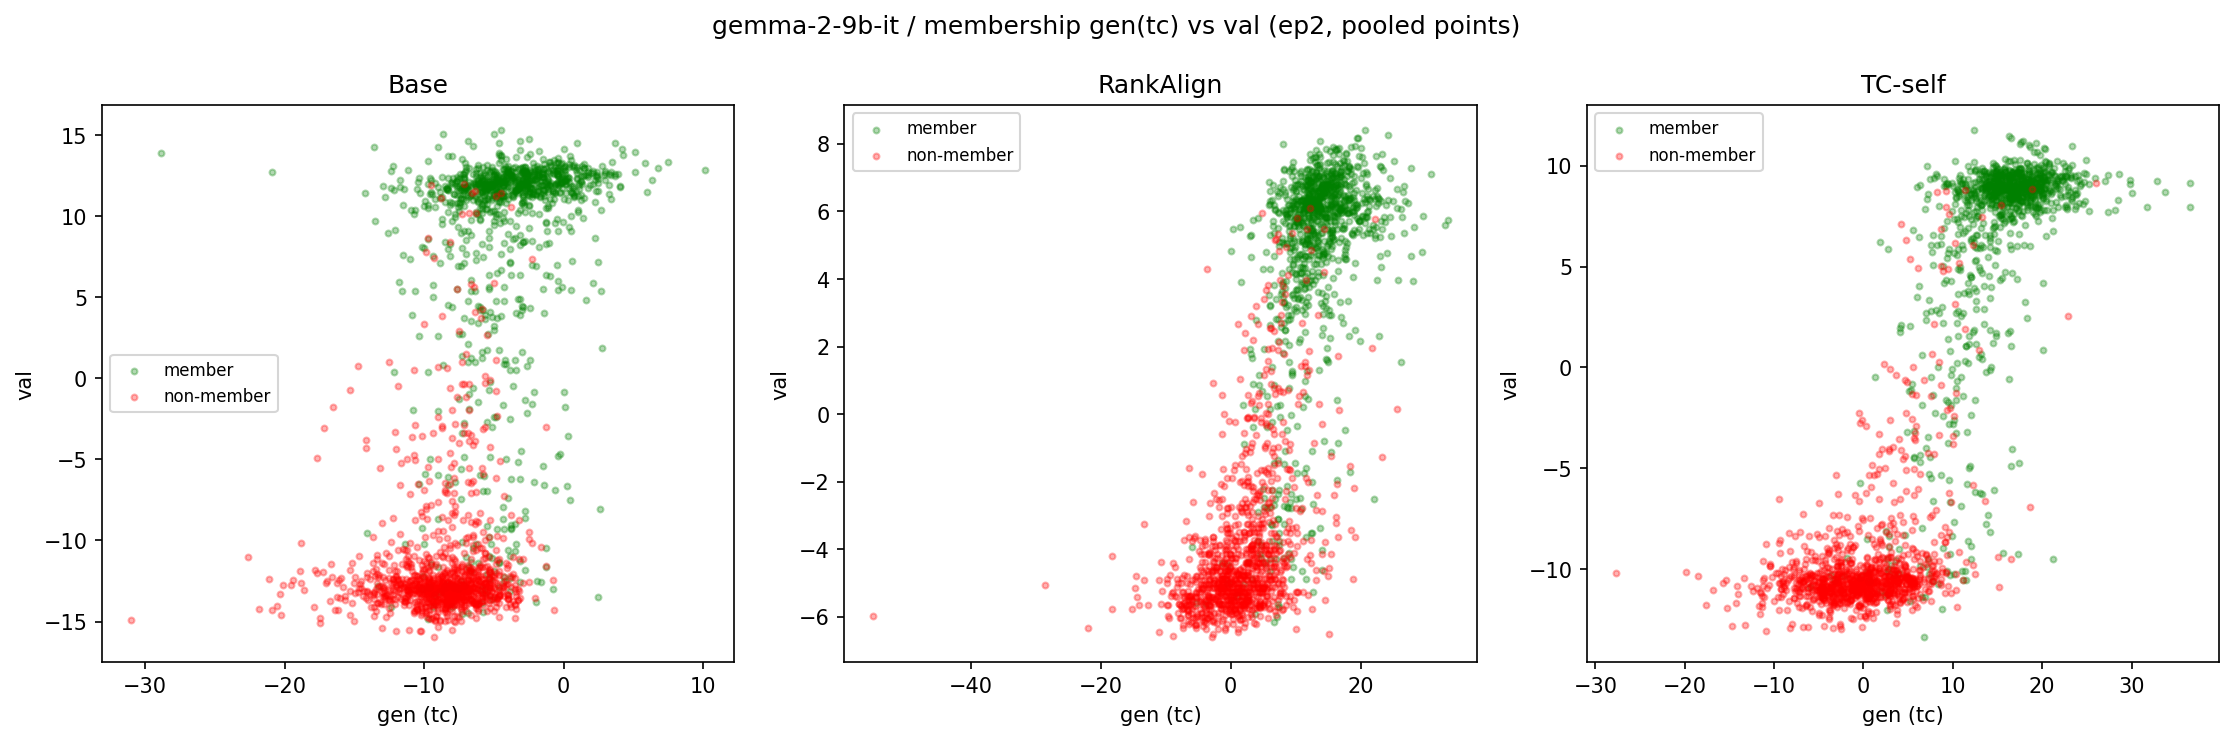
\includegraphics[width=0.95\textwidth]{plots/fix_gen_vs_val_scatter.png}
\caption{Generator (typicality-corrected) vs validator scores for Base, s2, and s4 (gemma
membership, ep2), pooling the raw candidate points (member green, non-member red) --- a raw
visualization, identical in procedure to the HumanEval report's scatter. Training improves the
member/non-member separation in both generator and validator space.}
\label{fig:scatter}
\end{figure}

\subsection{Per-Category Analysis}
\label{sec:percat}

\begin{figure}[H]
\centering
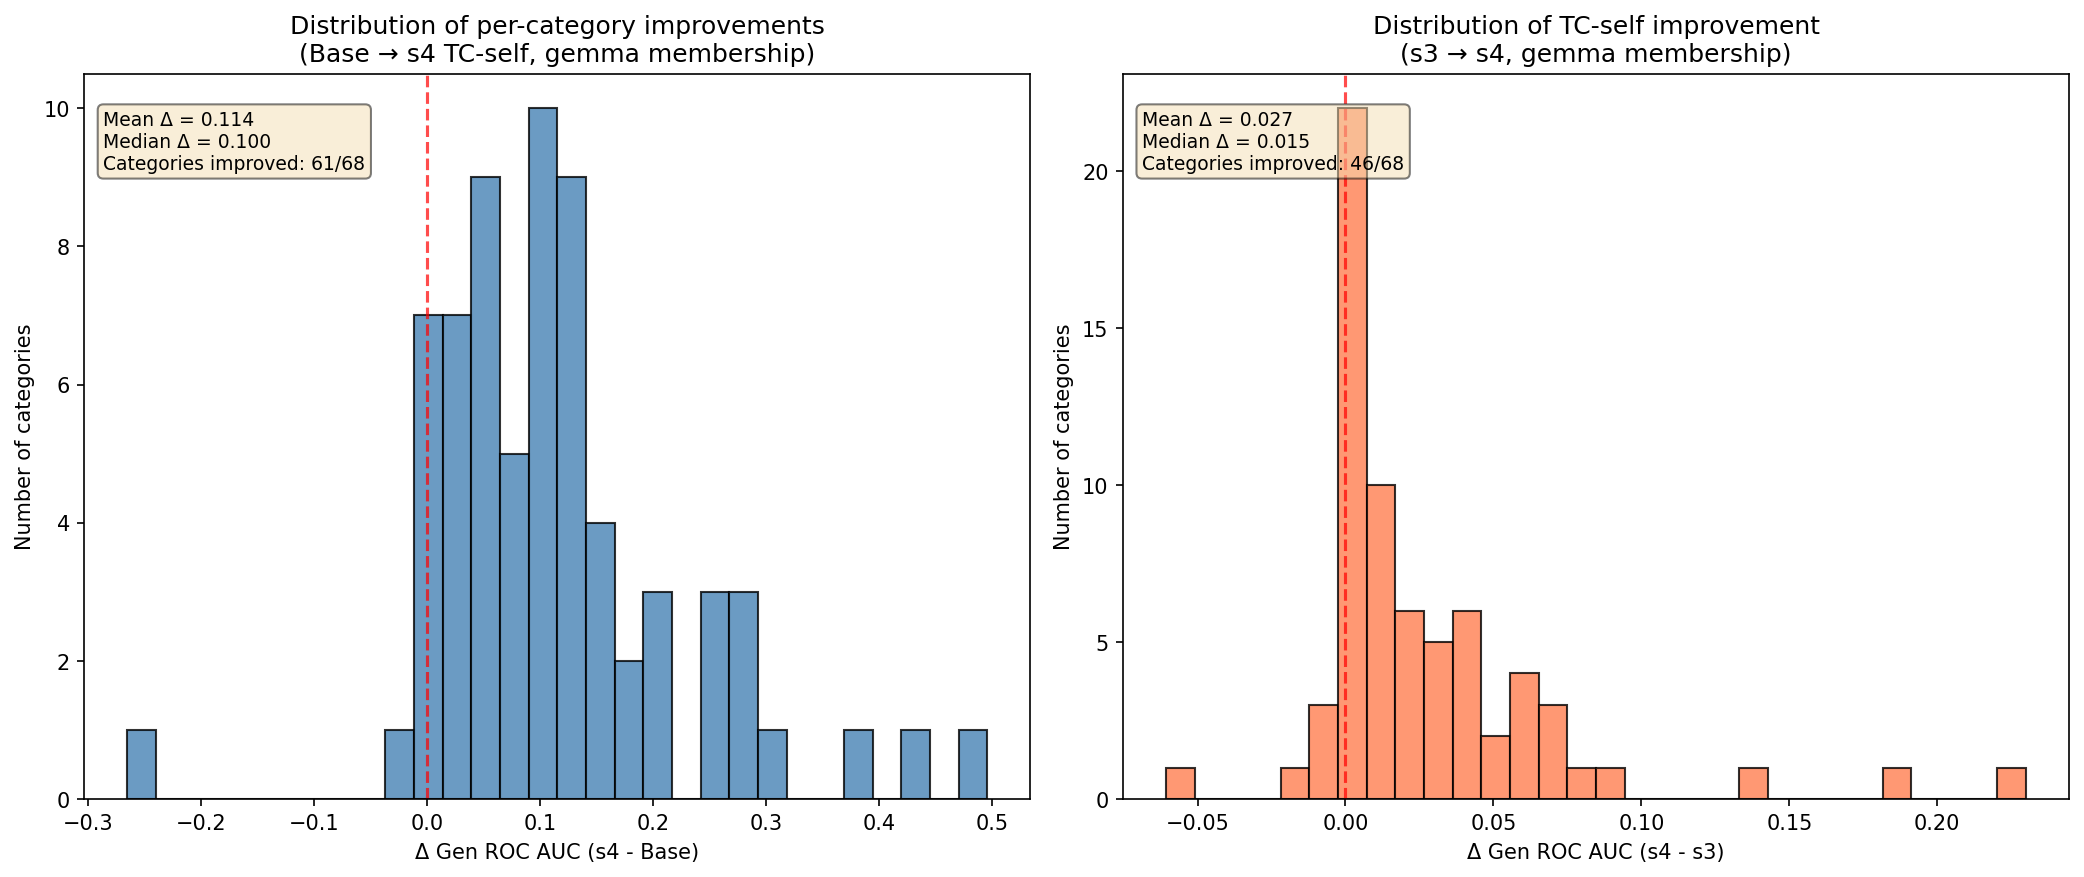
\includegraphics[width=0.95\textwidth]{plots/per_category_improvement_distribution.png}
\caption{Left: distribution of per-category improvements (Base $\to$ s4). Right: improvements from TC-self specifically (s3 $\to$ s4). Both are consistently positive.}
\label{fig:per_category}
\end{figure}

Categories where the base model was weakest (gen\_roc $\approx$ 0.5--0.7) benefit most from training. For example, ``medical specialty'' improves from 0.504 to 1.000 ($+$0.496). Categories already near ceiling show minimal gains (expected).

%% ============================================================
\section{Focused TC Comparison}
%% ============================================================

\subsection{Self-TC vs No-TC (s4 vs s3)}

When evaluated with self-TC scoring, the typicality-corrected models consistently outperform the non-TC baseline (s3):

\begin{itemize}
\item s4 (TC-self, full): $+0.028$ over s3
\item s6 (TC-self fsx, low $\delta$): $+0.023$ over s3
\item s11 (TC-self vlo, no fsx/ppd): $+0.022$ over s3
\item s5 (TC-self basic): $+0.010$ over s3
\end{itemize}

\subsection{Neg-TC vs No-TC (s7 vs s3)}

When evaluated with neg-TC scoring, the improvement from TC-neg training is even larger:

\begin{itemize}
\item s12 (TC-neg vlo): $+0.075$ over s3
\item s7 (TC-neg, full): $+0.072$ over s3
\end{itemize}

This suggests that TC-trained models learn better internal representations that are specifically captured by the matching TC scoring method.

\begin{figure}[H]
\centering
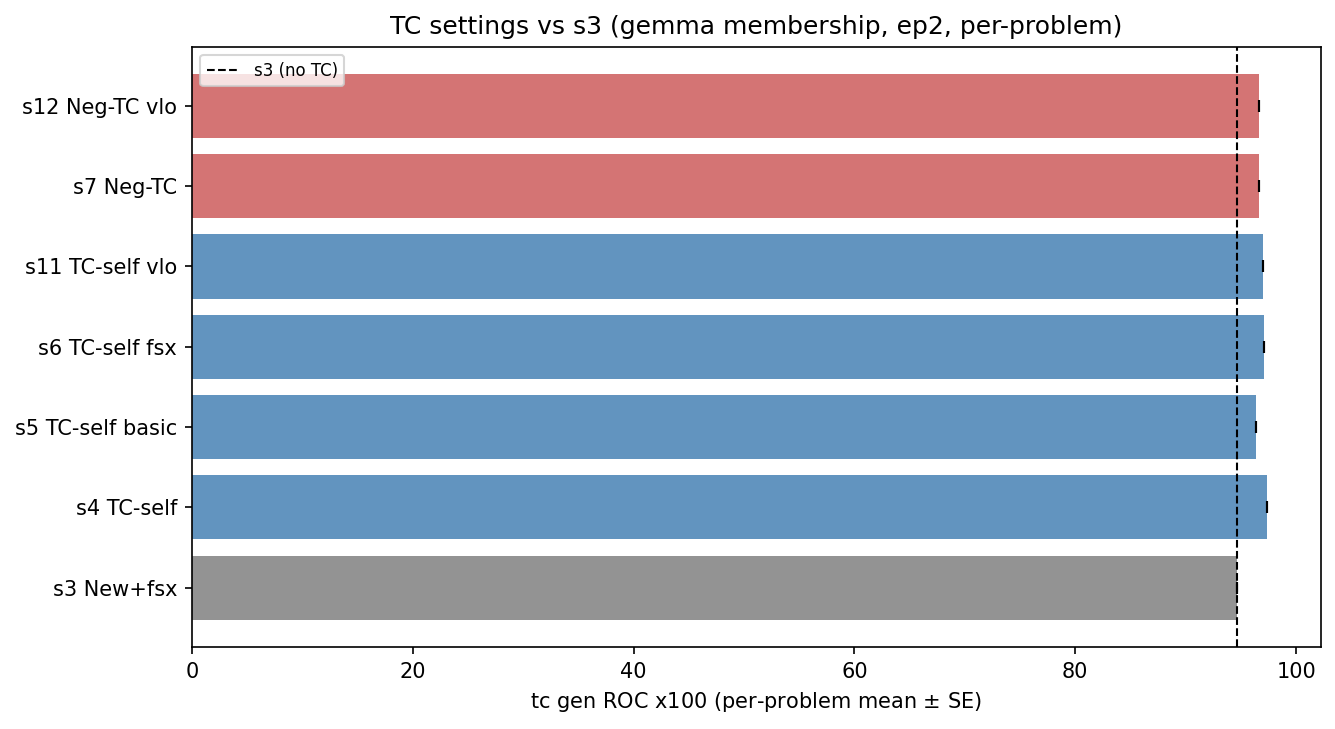
\includegraphics[width=0.95\textwidth]{plots/fix_tc_comparison.png}
\caption{TC comparison on gemma membership (ep2): per-problem typicality-corrected gen ROC
($\times100$, mean$\pm$SE) for the TC settings (self-TC: s4/s5/s6/s11; neg-TC: s7/s12) against the
no-TC s3 baseline (dashed). Same per-problem procedure as the HumanEval report.}
\label{fig:tc_comparison}
\end{figure}

\noindent The epoch-by-epoch dynamics for these settings are shown per problem in
Figure~\ref{fig:dynamics} (TC-trained models converge quickly and hold their advantage across
checkpoints).

%% ============================================================
\section{Train vs Test Generalization}
%% ============================================================

A critical finding emerges when comparing train-set dynamics with held-out test sets. Both panels
are gemma-2-9b-it, PMI-base (base-typicality) scoring, with \textbf{both train and test columns
computed per problem then averaged (mean$\pm$SE)} --- train on the model's own problems, test on
held-out problems of a different distribution. $\Delta=$ test$-$train.

\begin{table}[H]
\centering
\caption{Membership TRAIN (68 categories) vs.\ rosch TEST (10 held-out categories), per-category
mean$\pm$SE. s1 is shown only where both splits have it; s5/s11 are omitted (their per-category
rosch-test source no longer exists on disk and the raw s5/s11 rosch-test scores were not retained,
so they cannot be recomputed without re-evaluation); s7 (neg-TC) is excluded from this PMI-base
comparison.}
\label{tab:train_test}
% Auto-generated by build_report_fix_metrics.py (train-vs-test membership, per-problem PMI-base)
\begin{tabular}{lccc}
\toprule
\textbf{Setting} & \textbf{Train} & \textbf{Test (rosch)} & \textbf{$\Delta$} \\
\midrule
base & $0.860\se{0.014}$ & --- & --- \\
s2 & $0.945\se{0.007}$ & $0.895\se{0.015}$ & $-0.049$ \\
s3 & $0.947\se{0.011}$ & $0.886\se{0.012}$ & $-0.061$ \\
s4 & $0.974\se{0.009}$ & $0.926\se{0.013}$ & $-0.048$ \\
\bottomrule
\end{tabular}

\end{table}

\begin{table}[H]
\centering
\caption{IFEval TRAIN (79 prompts) vs.\ IFEval-OOD TEST (20 held-out prompts), per-prompt
mean$\pm$SE. PMI-base scoring (self-TC settings + base).}
\label{tab:train_test_ifeval}
% Auto-generated by build_report_fix_metrics.py (train-vs-test ifeval, per-problem PMI-base)
\begin{tabular}{lccc}
\toprule
\textbf{Setting} & \textbf{Train} & \textbf{Test (ifeval OOD)} & \textbf{$\Delta$} \\
\midrule
base & $0.792\se{0.018}$ & $0.783\se{0.022}$ & $-0.009$ \\
s1 & $0.646\se{0.025}$ & $0.582\se{0.040}$ & $-0.064$ \\
s2 & $0.491\se{0.022}$ & $0.434\se{0.048}$ & $-0.057$ \\
s3 & $0.841\se{0.016}$ & $0.785\se{0.034}$ & $-0.056$ \\
s4 & $0.837\se{0.016}$ & $0.806\se{0.025}$ & $-0.031$ \\
\bottomrule
\end{tabular}

\end{table}

\textbf{Key finding} (holds under per-problem recomputation): on membership/rosch, s3 (full method,
no TC) outperforms s2 on the training categories ($0.947$ vs $0.945$) but \emph{underperforms} on
the held-out rosch categories ($0.886$ vs $0.895$), while s4 (TC-self) is highest on both splits
($0.974$ train, $0.926$ test) --- \textbf{TC promotes generalization}. On IFEval, every setting
generalizes with only a small test drop (base $\Delta-0.009$, s4 $\Delta-0.031$), except basic
RankAlign (s2), which is near or below chance on \emph{both} train ($0.491$) and OOD test
($0.434$) --- it is simply broken on IFEval, not overfit.

\begin{figure}[H]
\centering
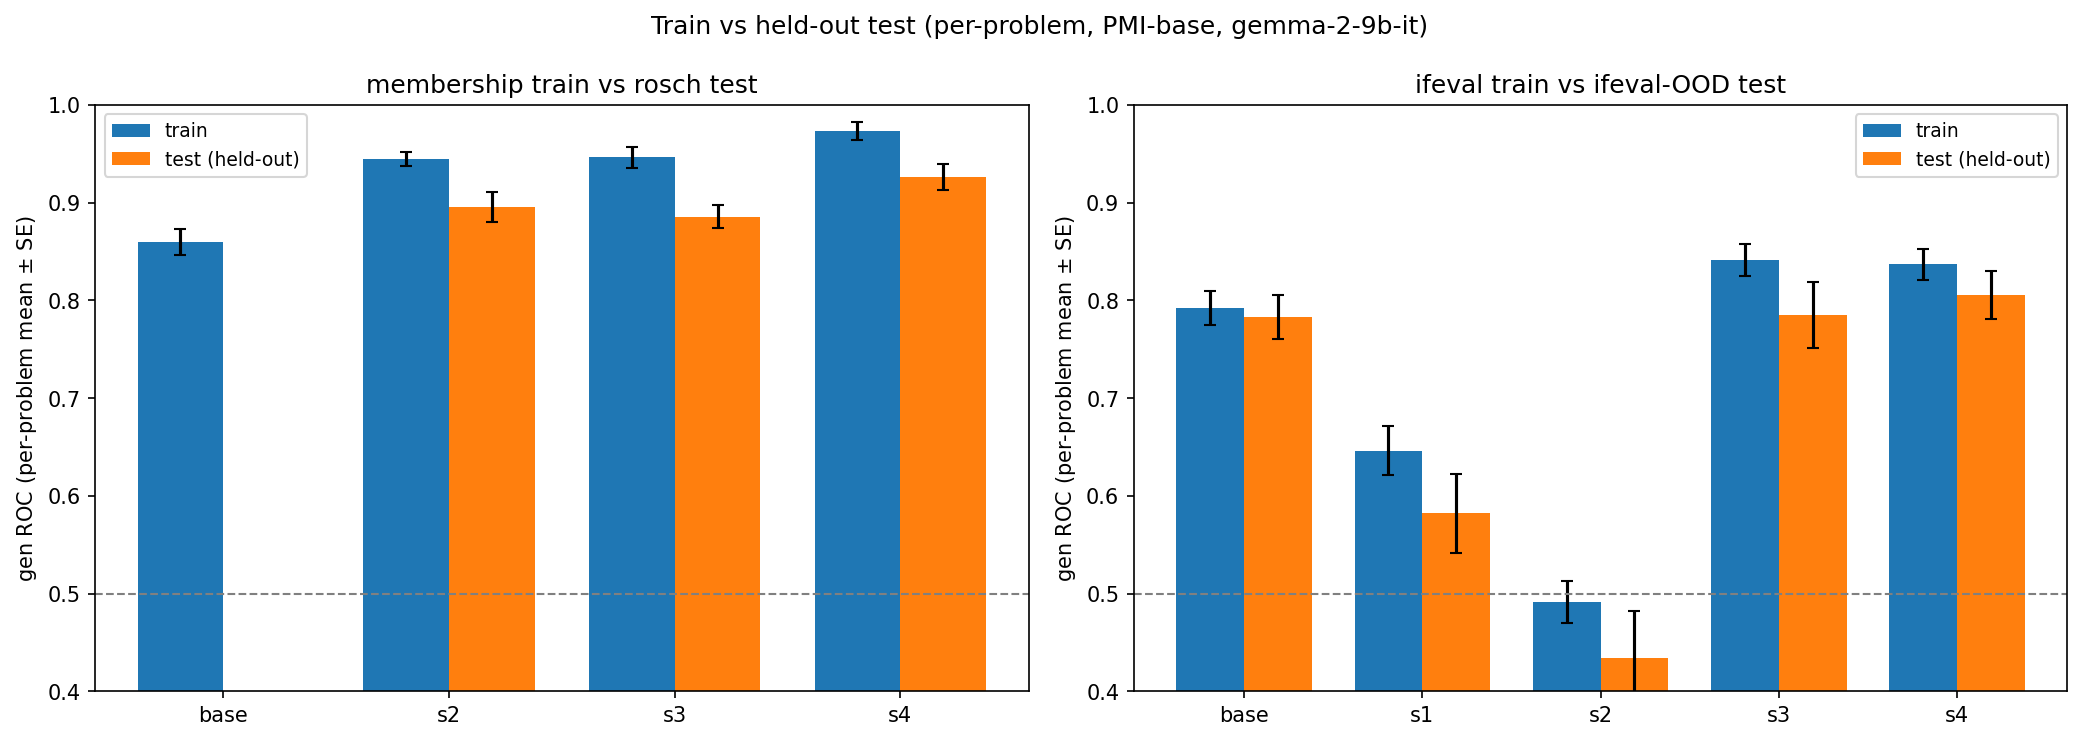
\includegraphics[width=0.95\textwidth]{plots/fix_train_vs_test.png}
\caption{Train vs held-out test gen ROC, \textbf{per-problem mean with SE error bars} (PMI-base,
gemma-2-9b-it). Left: membership train vs rosch test. Right: ifeval train vs ifeval-OOD test.
Dashed line is chance. Same per-problem procedure as the rest of this report.}
\label{fig:train_test}
\end{figure}

%% ============================================================
\section{Conclusions}
%% ============================================================

\begin{enumerate}
\item \textbf{RankAlign works when the full method (s3) is used} --- the NLL-V/G constraints are essential for preventing score explosion, especially on complex tasks like IFEval.
\item \textbf{TC-self training (s4) consistently provides the best results} across all metrics (gen ROC, spearman, concordance) and all model/task combinations.
\item \textbf{TC promotes generalization}: TC-trained models maintain their advantage on held-out test categories, while non-TC models (s3) can overfit to training patterns.
\item \textbf{Basic RankAlign (s2) is unreliable for complex tasks} --- it can actually \emph{hurt} performance (IFEval). The full method is needed.
\item \textbf{Score spread (gen\_delta\_mean) is a powerful training diagnostic} --- values $>$1000 indicate instability. TC-self produces the tightest distributions.
\item \textbf{Concordance is a complementary metric to ROC AUC} --- it directly measures the alignment between generator and validator ranking functions.
\end{enumerate}

\end{document}
